\documentclass[twoside]{book}

% Packages required by doxygen
\usepackage{fixltx2e}
\usepackage{calc}
\usepackage{doxygen}
\usepackage[export]{adjustbox} % also loads graphicx
\usepackage{graphicx}
\usepackage[utf8]{inputenc}
\usepackage{makeidx}
\usepackage{multicol}
\usepackage{multirow}
\PassOptionsToPackage{warn}{textcomp}
\usepackage{textcomp}
\usepackage[nointegrals]{wasysym}
\usepackage[table]{xcolor}

% Font selection
\usepackage[T1]{fontenc}
\usepackage[scaled=.90]{helvet}
\usepackage{courier}
\usepackage{amssymb}
\usepackage{sectsty}
\renewcommand{\familydefault}{\sfdefault}
\allsectionsfont{%
  \fontseries{bc}\selectfont%
  \color{darkgray}%
}
\renewcommand{\DoxyLabelFont}{%
  \fontseries{bc}\selectfont%
  \color{darkgray}%
}
\newcommand{\+}{\discretionary{\mbox{\scriptsize$\hookleftarrow$}}{}{}}

% Page & text layout
\usepackage{geometry}
\geometry{%
  a4paper,%
  top=2.5cm,%
  bottom=2.5cm,%
  left=2.5cm,%
  right=2.5cm%
}
\tolerance=750
\hfuzz=15pt
\hbadness=750
\setlength{\emergencystretch}{15pt}
\setlength{\parindent}{0cm}
\setlength{\parskip}{3ex plus 2ex minus 2ex}
\makeatletter
\renewcommand{\paragraph}{%
  \@startsection{paragraph}{4}{0ex}{-1.0ex}{1.0ex}{%
    \normalfont\normalsize\bfseries\SS@parafont%
  }%
}
\renewcommand{\subparagraph}{%
  \@startsection{subparagraph}{5}{0ex}{-1.0ex}{1.0ex}{%
    \normalfont\normalsize\bfseries\SS@subparafont%
  }%
}
\makeatother

% Headers & footers
\usepackage{fancyhdr}
\pagestyle{fancyplain}
\fancyhead[LE]{\fancyplain{}{\bfseries\thepage}}
\fancyhead[CE]{\fancyplain{}{}}
\fancyhead[RE]{\fancyplain{}{\bfseries\leftmark}}
\fancyhead[LO]{\fancyplain{}{\bfseries\rightmark}}
\fancyhead[CO]{\fancyplain{}{}}
\fancyhead[RO]{\fancyplain{}{\bfseries\thepage}}
\fancyfoot[LE]{\fancyplain{}{}}
\fancyfoot[CE]{\fancyplain{}{}}
\fancyfoot[RE]{\fancyplain{}{\bfseries\scriptsize Generated by Doxygen }}
\fancyfoot[LO]{\fancyplain{}{\bfseries\scriptsize Generated by Doxygen }}
\fancyfoot[CO]{\fancyplain{}{}}
\fancyfoot[RO]{\fancyplain{}{}}
\renewcommand{\footrulewidth}{0.4pt}
\renewcommand{\chaptermark}[1]{%
  \markboth{#1}{}%
}
\renewcommand{\sectionmark}[1]{%
  \markright{\thesection\ #1}%
}

% Indices & bibliography
\usepackage{natbib}
\usepackage[titles]{tocloft}
\setcounter{tocdepth}{3}
\setcounter{secnumdepth}{5}
\makeindex

% Hyperlinks (required, but should be loaded last)
\usepackage{ifpdf}
\ifpdf
  \usepackage[pdftex,pagebackref=true]{hyperref}
\else
  \usepackage[ps2pdf,pagebackref=true]{hyperref}
\fi
\hypersetup{%
  colorlinks=true,%
  linkcolor=blue,%
  citecolor=blue,%
  unicode%
}

% Custom commands
\newcommand{\clearemptydoublepage}{%
  \newpage{\pagestyle{empty}\cleardoublepage}%
}

\usepackage{caption}
\captionsetup{labelsep=space,justification=centering,font={bf},singlelinecheck=off,skip=4pt,position=top}

%===== C O N T E N T S =====

\begin{document}

% Titlepage & ToC
\hypersetup{pageanchor=false,
             bookmarksnumbered=true,
             pdfencoding=unicode
            }
\pagenumbering{alph}
\begin{titlepage}
\vspace*{7cm}
\begin{center}%
{\Large Rendu Style Novat }\\
\vspace*{1cm}
{\large Generated by Doxygen 1.8.15}\\
\end{center}
\end{titlepage}
\clearemptydoublepage
\pagenumbering{roman}
\tableofcontents
\clearemptydoublepage
\pagenumbering{arabic}
\hypersetup{pageanchor=true}

%--- Begin generated contents ---
\chapter{Hierarchical Index}
\section{Class Hierarchy}
This inheritance list is sorted roughly, but not completely, alphabetically\+:\begin{DoxyCompactList}
\item \contentsline{section}{Camera}{\pageref{class_camera}}{}
\item \contentsline{section}{Index}{\pageref{struct_index}}{}
\item \contentsline{section}{Mesh}{\pageref{class_mesh}}{}
\item \contentsline{section}{Mesh\+Loader}{\pageref{class_mesh_loader}}{}
\item \contentsline{section}{Model}{\pageref{class_model}}{}
\item Q\+Main\+Window\begin{DoxyCompactList}
\item \contentsline{section}{Main\+Window}{\pageref{class_main_window}}{}
\end{DoxyCompactList}
\item Q\+Object\begin{DoxyCompactList}
\item \contentsline{section}{Progress\+Info}{\pageref{class_progress_info}}{}
\end{DoxyCompactList}
\item Q\+Open\+G\+L\+Widget\begin{DoxyCompactList}
\item \contentsline{section}{Viewer}{\pageref{class_viewer}}{}
\end{DoxyCompactList}
\item \contentsline{section}{Shader}{\pageref{class_shader}}{}
\item \contentsline{section}{Texture}{\pageref{struct_texture}}{}
\item \contentsline{section}{Track\+Ball}{\pageref{class_track_ball}}{}
\item \contentsline{section}{Vertex}{\pageref{class_vertex}}{}
\end{DoxyCompactList}

\chapter{Class Index}
\section{Class List}
Here are the classes, structs, unions and interfaces with brief descriptions\+:\begin{DoxyCompactList}
\item\contentsline{section}{\mbox{\hyperlink{class_camera}{Camera}} \\*Define a camera link to a trackball for move the model arround the trackball. Compute model-\/view matrix, projection matrix and normal matrix. ! The center must be (0,0,0) (B\+UG) }{\pageref{class_camera}}{}
\item\contentsline{section}{\mbox{\hyperlink{struct_index}{Index}} }{\pageref{struct_index}}{}
\item\contentsline{section}{\mbox{\hyperlink{class_main_window}{Main\+Window}} \\*With basic menu bar (load model, save a screenshot and quit the app) and the central widget is a open\+Gl widget }{\pageref{class_main_window}}{}
\item\contentsline{section}{\mbox{\hyperlink{class_mesh}{Mesh}} \\*A \mbox{\hyperlink{class_mesh}{Mesh}} is a vector of vertex and a vector of int that define the indices of vertex of polygons of the mesh }{\pageref{class_mesh}}{}
\item\contentsline{section}{\mbox{\hyperlink{class_mesh_loader}{Mesh\+Loader}} \\*A class for loading a mesh from differentes files type }{\pageref{class_mesh_loader}}{}
\item\contentsline{section}{\mbox{\hyperlink{class_model}{Model}} \\*A model is defined by his mesh and his textures. It can load and draw a mesh and textures }{\pageref{class_model}}{}
\item\contentsline{section}{\mbox{\hyperlink{class_progress_info}{Progress\+Info}} \\*Store the information of a progress and emit 3 signal (begin, update and end) }{\pageref{class_progress_info}}{}
\item\contentsline{section}{\mbox{\hyperlink{class_shader}{Shader}} \\*The \mbox{\hyperlink{class_shader}{Shader}} class, opens, compiles and executes a vertex shader and a fragment shader }{\pageref{class_shader}}{}
\item\contentsline{section}{\mbox{\hyperlink{struct_texture}{Texture}} \\*A struct to store the id and the type of a texture }{\pageref{struct_texture}}{}
\item\contentsline{section}{\mbox{\hyperlink{class_track_ball}{Track\+Ball}} \\*A sphere that can move around his center }{\pageref{class_track_ball}}{}
\item\contentsline{section}{\mbox{\hyperlink{class_vertex}{Vertex}} \\*A Type class that define a vertex with his position , his normal and his texture coordinates }{\pageref{class_vertex}}{}
\item\contentsline{section}{\mbox{\hyperlink{class_viewer}{Viewer}} \\*The Open GL widget , init open\+GL, setup a model, a camera, a light and shaders and draw it }{\pageref{class_viewer}}{}
\end{DoxyCompactList}

\chapter{File Index}
\section{File List}
Here is a list of all documented files with brief descriptions\+:\begin{DoxyCompactList}
\item\contentsline{section}{src/\mbox{\hyperlink{camera_8h}{camera.\+h}} }{\pageref{camera_8h}}{}
\item\contentsline{section}{src/\mbox{\hyperlink{main_8cpp}{main.\+cpp}} \\*Application to generate a mountain panorama in the style of Pierre Novat }{\pageref{main_8cpp}}{}
\item\contentsline{section}{src/{\bfseries mainwindow.\+h} }{\pageref{mainwindow_8h}}{}
\item\contentsline{section}{src/{\bfseries mesh.\+h} }{\pageref{mesh_8h}}{}
\item\contentsline{section}{src/{\bfseries meshloader.\+h} }{\pageref{meshloader_8h}}{}
\item\contentsline{section}{src/{\bfseries model.\+h} }{\pageref{model_8h}}{}
\item\contentsline{section}{src/{\bfseries progressinfo.\+h} }{\pageref{progressinfo_8h}}{}
\item\contentsline{section}{src/{\bfseries shader.\+h} }{\pageref{shader_8h}}{}
\item\contentsline{section}{src/{\bfseries trackball.\+h} }{\pageref{trackball_8h}}{}
\item\contentsline{section}{src/{\bfseries vertex.\+h} }{\pageref{vertex_8h}}{}
\item\contentsline{section}{src/{\bfseries viewer.\+h} }{\pageref{viewer_8h}}{}
\end{DoxyCompactList}

\chapter{Class Documentation}
\hypertarget{class_camera}{}\section{Camera Class Reference}
\label{class_camera}\index{Camera@{Camera}}


Define a camera link to a trackball for move the model arround the trackball. Compute model-\/view matrix, projection matrix and normal matrix. ! The center must be (0,0,0) (B\+UG).  




{\ttfamily \#include $<$camera.\+h$>$}

\subsection*{Public Types}
\begin{DoxyCompactItemize}
\item 
\mbox{\Hypertarget{class_camera_a23162b5412510d749aad470789806872}\label{class_camera_a23162b5412510d749aad470789806872}} 
enum \{ {\bfseries N\+O\+NE}, 
{\bfseries R\+O\+T\+A\+TE}, 
{\bfseries M\+O\+V\+E\+XY}, 
{\bfseries M\+O\+V\+EZ}
 \}
\end{DoxyCompactItemize}
\subsection*{Public Member Functions}
\begin{DoxyCompactItemize}
\item 
\mbox{\hyperlink{class_camera_a9dcca190d009dad8bf772a7eee20c3b0}{Camera}} (float radius=1, const glm\+::vec3 \&center=glm\+::vec3(0, 0, 0), int mode=\mbox{\hyperlink{class_camera_a522ee90309c2918e4b9695fcdccd061c}{P\+E\+R\+SP}})
\item 
void \mbox{\hyperlink{class_camera_a01a5063edbbce200df991b5fd8761621}{initialize}} (int \mbox{\hyperlink{class_camera_a8695ceeb4597517ca9f2e09284f2506f}{w}}, int \mbox{\hyperlink{class_camera_a6a6e5717e8dd4bfaf6c9546a5cc09dc4}{h}}, bool replace=true)
\item 
void \mbox{\hyperlink{class_camera_ac21d2ee509fb8df94333a839b0892d54}{set\+Fovy}} (float f)
\item 
void \mbox{\hyperlink{class_camera_a9a436317f1a6e867f8eaa6affd6e80e5}{set\+Mode}} (int m)
\item 
void \mbox{\hyperlink{class_camera_af24fe5e14b2ba41196b95ad4a2eabb7c}{init\+Rotation}} (const glm\+::vec2 \&p)
\item 
void \mbox{\hyperlink{class_camera_a9f48e576aa251e716d97c32ac85bd7c4}{init\+Move\+XY}} (const glm\+::vec2 \&p)
\item 
void \mbox{\hyperlink{class_camera_a89c903f8ff8b16fccd8544af273ece2d}{init\+MoveZ}} (const glm\+::vec2 \&p)
\item 
void \mbox{\hyperlink{class_camera_a7ac215b4c76c1864c8c339127f4586ef}{move}} (const glm\+::vec2 \&p)
\item 
int \mbox{\hyperlink{class_camera_a8695ceeb4597517ca9f2e09284f2506f}{w}} () const
\item 
int \mbox{\hyperlink{class_camera_a6a6e5717e8dd4bfaf6c9546a5cc09dc4}{h}} () const
\item 
const glm\+::vec3 \mbox{\hyperlink{class_camera_adbbc2231e34b78b5b5b08a2aa16fc71d}{up}} () const
\item 
const glm\+::vec3 \mbox{\hyperlink{class_camera_a0f9545b5f7787ddc62f2d3a0f1e3c6d6}{right}} () const
\item 
const glm\+::vec3 \mbox{\hyperlink{class_camera_abbd1a0e73fd627b08d357524a7f1b8ab}{view}} () const
\item 
float \mbox{\hyperlink{class_camera_adf4779e2bc0dac7b719f4350c0db07f3}{zmin}} () const
\item 
float \mbox{\hyperlink{class_camera_a9f4ee36190bc2ef829efe11a8947dd5e}{zmax}} () const
\item 
float \mbox{\hyperlink{class_camera_ab437eb669d4bff47c4496933d06c5f9d}{fovy}} () const
\item 
const glm\+::vec2 \mbox{\hyperlink{class_camera_ae8cd001188c4b4381cd78a30f2669151}{pt}} () const
\item 
glm\+::mat4 \mbox{\hyperlink{class_camera_a30d3392172776022c53909e8b846995a}{proj\+Matrix}} () const
\item 
glm\+::mat4 \mbox{\hyperlink{class_camera_ac6671aeaa88d6cc673864f0183d5046b}{mdv\+Matrix}} () const
\item 
glm\+::mat3 \mbox{\hyperlink{class_camera_a2032bd7b990ca809759feabf2e54c612}{normal\+Matrix}} () const
\end{DoxyCompactItemize}
\subsection*{Static Public Attributes}
\begin{DoxyCompactItemize}
\item 
static const int \mbox{\hyperlink{class_camera_a522ee90309c2918e4b9695fcdccd061c}{P\+E\+R\+SP}} =0
\item 
static const int \mbox{\hyperlink{class_camera_a7244b2a4baebe084d16492758d16451c}{O\+R\+T\+HO}} =1
\end{DoxyCompactItemize}
\subsection*{Protected Member Functions}
\begin{DoxyCompactItemize}
\item 
void \mbox{\hyperlink{class_camera_a46f849a8ee9514d0e35269f5fce48096}{rotate}} (const glm\+::vec2 \&p)
\item 
void \mbox{\hyperlink{class_camera_a53a4ce8177d8622bcc01ae9a8f8fe391}{move\+XY}} (const glm\+::vec2 \&p)
\item 
void \mbox{\hyperlink{class_camera_a7c6676296255f1aef549228bf1c0a715}{moveZ}} (const glm\+::vec2 \&p)
\end{DoxyCompactItemize}


\subsection{Detailed Description}
Define a camera link to a trackball for move the model arround the trackball. Compute model-\/view matrix, projection matrix and normal matrix. ! The center must be (0,0,0) (B\+UG). 

\subsection{Constructor \& Destructor Documentation}
\mbox{\Hypertarget{class_camera_a9dcca190d009dad8bf772a7eee20c3b0}\label{class_camera_a9dcca190d009dad8bf772a7eee20c3b0}} 
\index{Camera@{Camera}!Camera@{Camera}}
\index{Camera@{Camera}!Camera@{Camera}}
\subsubsection{\texorpdfstring{Camera()}{Camera()}}
{\footnotesize\ttfamily Camera\+::\+Camera (\begin{DoxyParamCaption}\item[{float}]{radius = {\ttfamily 1},  }\item[{const glm\+::vec3 \&}]{center = {\ttfamily glm\+:\+:vec3(0,0,0)},  }\item[{int}]{mode = {\ttfamily \mbox{\hyperlink{class_camera_a522ee90309c2918e4b9695fcdccd061c}{P\+E\+R\+SP}}} }\end{DoxyParamCaption})}


\begin{DoxyParams}{Parameters}
{\em radius} & \\
\hline
{\em center} & \\
\hline
{\em mode} & \\
\hline
\end{DoxyParams}


\subsection{Member Function Documentation}
\mbox{\Hypertarget{class_camera_ab437eb669d4bff47c4496933d06c5f9d}\label{class_camera_ab437eb669d4bff47c4496933d06c5f9d}} 
\index{Camera@{Camera}!fovy@{fovy}}
\index{fovy@{fovy}!Camera@{Camera}}
\subsubsection{\texorpdfstring{fovy()}{fovy()}}
{\footnotesize\ttfamily float Camera\+::fovy (\begin{DoxyParamCaption}{ }\end{DoxyParamCaption}) const\hspace{0.3cm}{\ttfamily [inline]}}

\begin{DoxyReturn}{Returns}
float 
\end{DoxyReturn}
\mbox{\Hypertarget{class_camera_a6a6e5717e8dd4bfaf6c9546a5cc09dc4}\label{class_camera_a6a6e5717e8dd4bfaf6c9546a5cc09dc4}} 
\index{Camera@{Camera}!h@{h}}
\index{h@{h}!Camera@{Camera}}
\subsubsection{\texorpdfstring{h()}{h()}}
{\footnotesize\ttfamily int Camera\+::h (\begin{DoxyParamCaption}{ }\end{DoxyParamCaption}) const\hspace{0.3cm}{\ttfamily [inline]}}

\begin{DoxyReturn}{Returns}
int 
\end{DoxyReturn}
\mbox{\Hypertarget{class_camera_a01a5063edbbce200df991b5fd8761621}\label{class_camera_a01a5063edbbce200df991b5fd8761621}} 
\index{Camera@{Camera}!initialize@{initialize}}
\index{initialize@{initialize}!Camera@{Camera}}
\subsubsection{\texorpdfstring{initialize()}{initialize()}}
{\footnotesize\ttfamily void Camera\+::initialize (\begin{DoxyParamCaption}\item[{int}]{w,  }\item[{int}]{h,  }\item[{bool}]{replace = {\ttfamily true} }\end{DoxyParamCaption})}


\begin{DoxyParams}{Parameters}
{\em w} & \\
\hline
{\em h} & \\
\hline
{\em replace} & \\
\hline
\end{DoxyParams}
\mbox{\Hypertarget{class_camera_a9f48e576aa251e716d97c32ac85bd7c4}\label{class_camera_a9f48e576aa251e716d97c32ac85bd7c4}} 
\index{Camera@{Camera}!init\+Move\+XY@{init\+Move\+XY}}
\index{init\+Move\+XY@{init\+Move\+XY}!Camera@{Camera}}
\subsubsection{\texorpdfstring{init\+Move\+X\+Y()}{initMoveXY()}}
{\footnotesize\ttfamily void Camera\+::init\+Move\+XY (\begin{DoxyParamCaption}\item[{const glm\+::vec2 \&}]{p }\end{DoxyParamCaption})\hspace{0.3cm}{\ttfamily [inline]}}


\begin{DoxyParams}{Parameters}
{\em p} & \\
\hline
\end{DoxyParams}
\mbox{\Hypertarget{class_camera_a89c903f8ff8b16fccd8544af273ece2d}\label{class_camera_a89c903f8ff8b16fccd8544af273ece2d}} 
\index{Camera@{Camera}!init\+MoveZ@{init\+MoveZ}}
\index{init\+MoveZ@{init\+MoveZ}!Camera@{Camera}}
\subsubsection{\texorpdfstring{init\+Move\+Z()}{initMoveZ()}}
{\footnotesize\ttfamily void Camera\+::init\+MoveZ (\begin{DoxyParamCaption}\item[{const glm\+::vec2 \&}]{p }\end{DoxyParamCaption})\hspace{0.3cm}{\ttfamily [inline]}}


\begin{DoxyParams}{Parameters}
{\em p} & \\
\hline
\end{DoxyParams}
\mbox{\Hypertarget{class_camera_af24fe5e14b2ba41196b95ad4a2eabb7c}\label{class_camera_af24fe5e14b2ba41196b95ad4a2eabb7c}} 
\index{Camera@{Camera}!init\+Rotation@{init\+Rotation}}
\index{init\+Rotation@{init\+Rotation}!Camera@{Camera}}
\subsubsection{\texorpdfstring{init\+Rotation()}{initRotation()}}
{\footnotesize\ttfamily void Camera\+::init\+Rotation (\begin{DoxyParamCaption}\item[{const glm\+::vec2 \&}]{p }\end{DoxyParamCaption})\hspace{0.3cm}{\ttfamily [inline]}}


\begin{DoxyParams}{Parameters}
{\em p} & \\
\hline
\end{DoxyParams}
\mbox{\Hypertarget{class_camera_ac6671aeaa88d6cc673864f0183d5046b}\label{class_camera_ac6671aeaa88d6cc673864f0183d5046b}} 
\index{Camera@{Camera}!mdv\+Matrix@{mdv\+Matrix}}
\index{mdv\+Matrix@{mdv\+Matrix}!Camera@{Camera}}
\subsubsection{\texorpdfstring{mdv\+Matrix()}{mdvMatrix()}}
{\footnotesize\ttfamily glm\+::mat4 Camera\+::mdv\+Matrix (\begin{DoxyParamCaption}{ }\end{DoxyParamCaption}) const\hspace{0.3cm}{\ttfamily [inline]}}

\begin{DoxyReturn}{Returns}
glm\+::mat4 
\end{DoxyReturn}
\mbox{\Hypertarget{class_camera_a7ac215b4c76c1864c8c339127f4586ef}\label{class_camera_a7ac215b4c76c1864c8c339127f4586ef}} 
\index{Camera@{Camera}!move@{move}}
\index{move@{move}!Camera@{Camera}}
\subsubsection{\texorpdfstring{move()}{move()}}
{\footnotesize\ttfamily void Camera\+::move (\begin{DoxyParamCaption}\item[{const glm\+::vec2 \&}]{p }\end{DoxyParamCaption})\hspace{0.3cm}{\ttfamily [inline]}}


\begin{DoxyParams}{Parameters}
{\em p} & \\
\hline
\end{DoxyParams}
\mbox{\Hypertarget{class_camera_a53a4ce8177d8622bcc01ae9a8f8fe391}\label{class_camera_a53a4ce8177d8622bcc01ae9a8f8fe391}} 
\index{Camera@{Camera}!move\+XY@{move\+XY}}
\index{move\+XY@{move\+XY}!Camera@{Camera}}
\subsubsection{\texorpdfstring{move\+X\+Y()}{moveXY()}}
{\footnotesize\ttfamily void Camera\+::move\+XY (\begin{DoxyParamCaption}\item[{const glm\+::vec2 \&}]{p }\end{DoxyParamCaption})\hspace{0.3cm}{\ttfamily [inline]}, {\ttfamily [protected]}}


\begin{DoxyParams}{Parameters}
{\em p} & \\
\hline
\end{DoxyParams}
\mbox{\Hypertarget{class_camera_a7c6676296255f1aef549228bf1c0a715}\label{class_camera_a7c6676296255f1aef549228bf1c0a715}} 
\index{Camera@{Camera}!moveZ@{moveZ}}
\index{moveZ@{moveZ}!Camera@{Camera}}
\subsubsection{\texorpdfstring{move\+Z()}{moveZ()}}
{\footnotesize\ttfamily void Camera\+::moveZ (\begin{DoxyParamCaption}\item[{const glm\+::vec2 \&}]{p }\end{DoxyParamCaption})\hspace{0.3cm}{\ttfamily [inline]}, {\ttfamily [protected]}}


\begin{DoxyParams}{Parameters}
{\em p} & \\
\hline
\end{DoxyParams}
\mbox{\Hypertarget{class_camera_a2032bd7b990ca809759feabf2e54c612}\label{class_camera_a2032bd7b990ca809759feabf2e54c612}} 
\index{Camera@{Camera}!normal\+Matrix@{normal\+Matrix}}
\index{normal\+Matrix@{normal\+Matrix}!Camera@{Camera}}
\subsubsection{\texorpdfstring{normal\+Matrix()}{normalMatrix()}}
{\footnotesize\ttfamily glm\+::mat3 Camera\+::normal\+Matrix (\begin{DoxyParamCaption}{ }\end{DoxyParamCaption}) const\hspace{0.3cm}{\ttfamily [inline]}}

\begin{DoxyReturn}{Returns}
glm\+::mat3 
\end{DoxyReturn}
\mbox{\Hypertarget{class_camera_a30d3392172776022c53909e8b846995a}\label{class_camera_a30d3392172776022c53909e8b846995a}} 
\index{Camera@{Camera}!proj\+Matrix@{proj\+Matrix}}
\index{proj\+Matrix@{proj\+Matrix}!Camera@{Camera}}
\subsubsection{\texorpdfstring{proj\+Matrix()}{projMatrix()}}
{\footnotesize\ttfamily glm\+::mat4 Camera\+::proj\+Matrix (\begin{DoxyParamCaption}{ }\end{DoxyParamCaption}) const\hspace{0.3cm}{\ttfamily [inline]}}

\begin{DoxyReturn}{Returns}
glm\+::mat4 
\end{DoxyReturn}
\mbox{\Hypertarget{class_camera_ae8cd001188c4b4381cd78a30f2669151}\label{class_camera_ae8cd001188c4b4381cd78a30f2669151}} 
\index{Camera@{Camera}!pt@{pt}}
\index{pt@{pt}!Camera@{Camera}}
\subsubsection{\texorpdfstring{pt()}{pt()}}
{\footnotesize\ttfamily const glm\+::vec2 Camera\+::pt (\begin{DoxyParamCaption}{ }\end{DoxyParamCaption}) const\hspace{0.3cm}{\ttfamily [inline]}}

\begin{DoxyReturn}{Returns}
const glm\+::vec2 
\end{DoxyReturn}
\mbox{\Hypertarget{class_camera_a0f9545b5f7787ddc62f2d3a0f1e3c6d6}\label{class_camera_a0f9545b5f7787ddc62f2d3a0f1e3c6d6}} 
\index{Camera@{Camera}!right@{right}}
\index{right@{right}!Camera@{Camera}}
\subsubsection{\texorpdfstring{right()}{right()}}
{\footnotesize\ttfamily const glm\+::vec3 Camera\+::right (\begin{DoxyParamCaption}{ }\end{DoxyParamCaption}) const\hspace{0.3cm}{\ttfamily [inline]}}

\begin{DoxyReturn}{Returns}
const glm\+::vec3 
\end{DoxyReturn}
\mbox{\Hypertarget{class_camera_a46f849a8ee9514d0e35269f5fce48096}\label{class_camera_a46f849a8ee9514d0e35269f5fce48096}} 
\index{Camera@{Camera}!rotate@{rotate}}
\index{rotate@{rotate}!Camera@{Camera}}
\subsubsection{\texorpdfstring{rotate()}{rotate()}}
{\footnotesize\ttfamily void Camera\+::rotate (\begin{DoxyParamCaption}\item[{const glm\+::vec2 \&}]{p }\end{DoxyParamCaption})\hspace{0.3cm}{\ttfamily [inline]}, {\ttfamily [protected]}}


\begin{DoxyParams}{Parameters}
{\em p} & \\
\hline
\end{DoxyParams}
\mbox{\Hypertarget{class_camera_ac21d2ee509fb8df94333a839b0892d54}\label{class_camera_ac21d2ee509fb8df94333a839b0892d54}} 
\index{Camera@{Camera}!set\+Fovy@{set\+Fovy}}
\index{set\+Fovy@{set\+Fovy}!Camera@{Camera}}
\subsubsection{\texorpdfstring{set\+Fovy()}{setFovy()}}
{\footnotesize\ttfamily void Camera\+::set\+Fovy (\begin{DoxyParamCaption}\item[{float}]{f }\end{DoxyParamCaption})}


\begin{DoxyParams}{Parameters}
{\em f} & \\
\hline
\end{DoxyParams}
\mbox{\Hypertarget{class_camera_a9a436317f1a6e867f8eaa6affd6e80e5}\label{class_camera_a9a436317f1a6e867f8eaa6affd6e80e5}} 
\index{Camera@{Camera}!set\+Mode@{set\+Mode}}
\index{set\+Mode@{set\+Mode}!Camera@{Camera}}
\subsubsection{\texorpdfstring{set\+Mode()}{setMode()}}
{\footnotesize\ttfamily void Camera\+::set\+Mode (\begin{DoxyParamCaption}\item[{int}]{m }\end{DoxyParamCaption})}


\begin{DoxyParams}{Parameters}
{\em m} & \\
\hline
\end{DoxyParams}
\mbox{\Hypertarget{class_camera_adbbc2231e34b78b5b5b08a2aa16fc71d}\label{class_camera_adbbc2231e34b78b5b5b08a2aa16fc71d}} 
\index{Camera@{Camera}!up@{up}}
\index{up@{up}!Camera@{Camera}}
\subsubsection{\texorpdfstring{up()}{up()}}
{\footnotesize\ttfamily const glm\+::vec3 Camera\+::up (\begin{DoxyParamCaption}{ }\end{DoxyParamCaption}) const\hspace{0.3cm}{\ttfamily [inline]}}

\begin{DoxyReturn}{Returns}
const glm\+::vec3 
\end{DoxyReturn}
\mbox{\Hypertarget{class_camera_abbd1a0e73fd627b08d357524a7f1b8ab}\label{class_camera_abbd1a0e73fd627b08d357524a7f1b8ab}} 
\index{Camera@{Camera}!view@{view}}
\index{view@{view}!Camera@{Camera}}
\subsubsection{\texorpdfstring{view()}{view()}}
{\footnotesize\ttfamily const glm\+::vec3 Camera\+::view (\begin{DoxyParamCaption}{ }\end{DoxyParamCaption}) const\hspace{0.3cm}{\ttfamily [inline]}}

\begin{DoxyReturn}{Returns}
const glm\+::vec3 
\end{DoxyReturn}
\mbox{\Hypertarget{class_camera_a8695ceeb4597517ca9f2e09284f2506f}\label{class_camera_a8695ceeb4597517ca9f2e09284f2506f}} 
\index{Camera@{Camera}!w@{w}}
\index{w@{w}!Camera@{Camera}}
\subsubsection{\texorpdfstring{w()}{w()}}
{\footnotesize\ttfamily int Camera\+::w (\begin{DoxyParamCaption}{ }\end{DoxyParamCaption}) const\hspace{0.3cm}{\ttfamily [inline]}}

\begin{DoxyReturn}{Returns}
int 
\end{DoxyReturn}
\mbox{\Hypertarget{class_camera_a9f4ee36190bc2ef829efe11a8947dd5e}\label{class_camera_a9f4ee36190bc2ef829efe11a8947dd5e}} 
\index{Camera@{Camera}!zmax@{zmax}}
\index{zmax@{zmax}!Camera@{Camera}}
\subsubsection{\texorpdfstring{zmax()}{zmax()}}
{\footnotesize\ttfamily float Camera\+::zmax (\begin{DoxyParamCaption}{ }\end{DoxyParamCaption}) const\hspace{0.3cm}{\ttfamily [inline]}}

\begin{DoxyReturn}{Returns}
float 
\end{DoxyReturn}
\mbox{\Hypertarget{class_camera_adf4779e2bc0dac7b719f4350c0db07f3}\label{class_camera_adf4779e2bc0dac7b719f4350c0db07f3}} 
\index{Camera@{Camera}!zmin@{zmin}}
\index{zmin@{zmin}!Camera@{Camera}}
\subsubsection{\texorpdfstring{zmin()}{zmin()}}
{\footnotesize\ttfamily float Camera\+::zmin (\begin{DoxyParamCaption}{ }\end{DoxyParamCaption}) const\hspace{0.3cm}{\ttfamily [inline]}}

\begin{DoxyReturn}{Returns}
float 
\end{DoxyReturn}


\subsection{Member Data Documentation}
\mbox{\Hypertarget{class_camera_a7244b2a4baebe084d16492758d16451c}\label{class_camera_a7244b2a4baebe084d16492758d16451c}} 
\index{Camera@{Camera}!O\+R\+T\+HO@{O\+R\+T\+HO}}
\index{O\+R\+T\+HO@{O\+R\+T\+HO}!Camera@{Camera}}
\subsubsection{\texorpdfstring{O\+R\+T\+HO}{ORTHO}}
{\footnotesize\ttfamily const int Camera\+::\+O\+R\+T\+HO =1\hspace{0.3cm}{\ttfamily [static]}}

T\+O\+DO\+: describe \mbox{\Hypertarget{class_camera_a522ee90309c2918e4b9695fcdccd061c}\label{class_camera_a522ee90309c2918e4b9695fcdccd061c}} 
\index{Camera@{Camera}!P\+E\+R\+SP@{P\+E\+R\+SP}}
\index{P\+E\+R\+SP@{P\+E\+R\+SP}!Camera@{Camera}}
\subsubsection{\texorpdfstring{P\+E\+R\+SP}{PERSP}}
{\footnotesize\ttfamily const int Camera\+::\+P\+E\+R\+SP =0\hspace{0.3cm}{\ttfamily [static]}}

T\+O\+DO\+: describe 

The documentation for this class was generated from the following files\+:\begin{DoxyCompactItemize}
\item 
src/\mbox{\hyperlink{camera_8h}{camera.\+h}}\item 
src/camera.\+cpp\end{DoxyCompactItemize}

\hypertarget{struct_index}{}\section{Index Struct Reference}
\label{struct_index}\index{Index@{Index}}
\subsection*{Public Attributes}
\begin{DoxyCompactItemize}
\item 
\mbox{\Hypertarget{struct_index_a19da745bad3ef10f056deb1d5c847977}\label{struct_index_a19da745bad3ef10f056deb1d5c847977}} 
int {\bfseries position}
\item 
\mbox{\Hypertarget{struct_index_a426230d3d71ced90862af80a6beabcf3}\label{struct_index_a426230d3d71ced90862af80a6beabcf3}} 
int {\bfseries normal}
\item 
\mbox{\Hypertarget{struct_index_ae033ccddebcd55920d047fdb180ed6ff}\label{struct_index_ae033ccddebcd55920d047fdb180ed6ff}} 
int {\bfseries tex\+Coord}
\item 
\mbox{\Hypertarget{struct_index_a070fb177b4763f7e90f175c7784d81ee}\label{struct_index_a070fb177b4763f7e90f175c7784d81ee}} 
int {\bfseries indice}
\end{DoxyCompactItemize}


The documentation for this struct was generated from the following file\+:\begin{DoxyCompactItemize}
\item 
src/Indexation\+\_\+test.\+cpp\end{DoxyCompactItemize}

\hypertarget{class_main_window}{}\section{Main\+Window Class Reference}
\label{class_main_window}\index{Main\+Window@{Main\+Window}}


The \mbox{\hyperlink{class_main_window}{Main\+Window}} class with basic menu bar (load model, save a screenshot and quit the app) and the central widget is a open\+Gl widget.  




{\ttfamily \#include $<$mainwindow.\+h$>$}



Inheritance diagram for Main\+Window\+:
\nopagebreak
\begin{figure}[H]
\begin{center}
\leavevmode
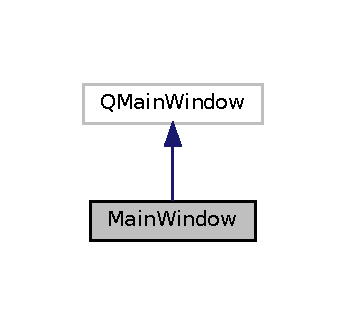
\includegraphics[width=166pt]{class_main_window__inherit__graph}
\end{center}
\end{figure}


Collaboration diagram for Main\+Window\+:
\nopagebreak
\begin{figure}[H]
\begin{center}
\leavevmode
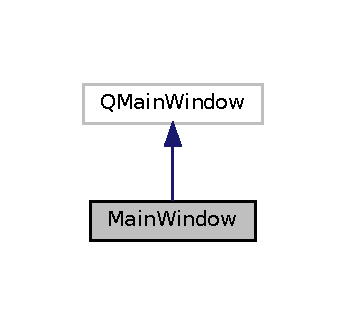
\includegraphics[width=166pt]{class_main_window__coll__graph}
\end{center}
\end{figure}
\subsection*{Public Member Functions}
\begin{DoxyCompactItemize}
\item 
\mbox{\Hypertarget{class_main_window_a34c4b4207b46d11a4100c9b19f0e81bb}\label{class_main_window_a34c4b4207b46d11a4100c9b19f0e81bb}} 
\mbox{\hyperlink{class_main_window_a34c4b4207b46d11a4100c9b19f0e81bb}{Main\+Window}} ()
\begin{DoxyCompactList}\small\item\em Set the different Widget. \end{DoxyCompactList}\end{DoxyCompactItemize}
\subsection*{Protected Member Functions}
\begin{DoxyCompactItemize}
\item 
void \mbox{\hyperlink{class_main_window_a05fb9d72c044aa3bb7d187b994704e2f}{close\+Event}} (Q\+Close\+Event $\ast$event) override
\begin{DoxyCompactList}\small\item\em Intercepts the close\+Event and destroy all the variable of main\+Window. \end{DoxyCompactList}\end{DoxyCompactItemize}


\subsection{Detailed Description}
The \mbox{\hyperlink{class_main_window}{Main\+Window}} class with basic menu bar (load model, save a screenshot and quit the app) and the central widget is a open\+Gl widget. 

\subsection{Member Function Documentation}
\mbox{\Hypertarget{class_main_window_a05fb9d72c044aa3bb7d187b994704e2f}\label{class_main_window_a05fb9d72c044aa3bb7d187b994704e2f}} 
\index{Main\+Window@{Main\+Window}!close\+Event@{close\+Event}}
\index{close\+Event@{close\+Event}!Main\+Window@{Main\+Window}}
\subsubsection{\texorpdfstring{close\+Event()}{closeEvent()}}
{\footnotesize\ttfamily void Main\+Window\+::close\+Event (\begin{DoxyParamCaption}\item[{Q\+Close\+Event $\ast$}]{event }\end{DoxyParamCaption})\hspace{0.3cm}{\ttfamily [override]}, {\ttfamily [protected]}}



Intercepts the close\+Event and destroy all the variable of main\+Window. 


\begin{DoxyParams}{Parameters}
{\em event} & \\
\hline
\end{DoxyParams}


The documentation for this class was generated from the following files\+:\begin{DoxyCompactItemize}
\item 
src/mainwindow.\+h\item 
src/mainwindow.\+cpp\end{DoxyCompactItemize}

\hypertarget{class_mesh}{}\section{Mesh Class Reference}
\label{class_mesh}\index{Mesh@{Mesh}}


A \mbox{\hyperlink{class_mesh}{Mesh}} is a vector of vertex and a vector of int that define the indices of vertex of polygons of the mesh.  




{\ttfamily \#include $<$mesh.\+h$>$}

\subsection*{Public Member Functions}
\begin{DoxyCompactItemize}
\item 
\mbox{\hyperlink{class_mesh_a9471cc66749be2d05a9e2bdf77090450}{Mesh}} (std\+::vector$<$ \mbox{\hyperlink{class_vertex}{Vertex}} $>$ vertices, std\+::vector$<$ unsigned int $>$ indices)
\begin{DoxyCompactList}\small\item\em set \+\_\+vertices and \+\_\+indices and start setup\+Mesh. \end{DoxyCompactList}\item 
\mbox{\Hypertarget{class_mesh_afdd95c079fd0442afef8a6c421c8bfc9}\label{class_mesh_afdd95c079fd0442afef8a6c421c8bfc9}} 
void \mbox{\hyperlink{class_mesh_afdd95c079fd0442afef8a6c421c8bfc9}{Draw}} ()
\begin{DoxyCompactList}\small\item\em Draw the mesh. \end{DoxyCompactList}\item 
\mbox{\Hypertarget{class_mesh_aafa4e21067a9b0c4407daf5e3c9ea991}\label{class_mesh_aafa4e21067a9b0c4407daf5e3c9ea991}} 
void \mbox{\hyperlink{class_mesh_aafa4e21067a9b0c4407daf5e3c9ea991}{setup\+Mesh}} ()
\begin{DoxyCompactList}\small\item\em load the mesh data into the G\+PU with a V\+AO, V\+BO and E\+BO. \end{DoxyCompactList}\end{DoxyCompactItemize}
\subsection*{Public Attributes}
\begin{DoxyCompactItemize}
\item 
\mbox{\Hypertarget{class_mesh_ac8bc82604ad2b353e0f3f22edb166960}\label{class_mesh_ac8bc82604ad2b353e0f3f22edb166960}} 
std\+::vector$<$ \mbox{\hyperlink{class_vertex}{Vertex}} $>$ \mbox{\hyperlink{class_mesh_ac8bc82604ad2b353e0f3f22edb166960}{\+\_\+vertices}}
\begin{DoxyCompactList}\small\item\em a vector of vertex. \end{DoxyCompactList}\item 
\mbox{\Hypertarget{class_mesh_a79f0d5bbd4dba6a7f6cb3b9eb6854ddf}\label{class_mesh_a79f0d5bbd4dba6a7f6cb3b9eb6854ddf}} 
std\+::vector$<$ unsigned int $>$ \mbox{\hyperlink{class_mesh_a79f0d5bbd4dba6a7f6cb3b9eb6854ddf}{\+\_\+indices}}
\begin{DoxyCompactList}\small\item\em a vector of int that define the indices of vertex of polygons of the mesh. \end{DoxyCompactList}\item 
\mbox{\Hypertarget{class_mesh_a88114ad56bdd0ff198a39aaf7c5ea12e}\label{class_mesh_a88114ad56bdd0ff198a39aaf7c5ea12e}} 
unsigned int \mbox{\hyperlink{class_mesh_a88114ad56bdd0ff198a39aaf7c5ea12e}{\+\_\+\+V\+AO}}
\begin{DoxyCompactList}\small\item\em a \mbox{\hyperlink{class_vertex}{Vertex}} Array Object. \end{DoxyCompactList}\end{DoxyCompactItemize}


\subsection{Detailed Description}
A \mbox{\hyperlink{class_mesh}{Mesh}} is a vector of vertex and a vector of int that define the indices of vertex of polygons of the mesh. 

\subsection{Constructor \& Destructor Documentation}
\mbox{\Hypertarget{class_mesh_a9471cc66749be2d05a9e2bdf77090450}\label{class_mesh_a9471cc66749be2d05a9e2bdf77090450}} 
\index{Mesh@{Mesh}!Mesh@{Mesh}}
\index{Mesh@{Mesh}!Mesh@{Mesh}}
\subsubsection{\texorpdfstring{Mesh()}{Mesh()}}
{\footnotesize\ttfamily Mesh\+::\+Mesh (\begin{DoxyParamCaption}\item[{std\+::vector$<$ \mbox{\hyperlink{class_vertex}{Vertex}} $>$}]{vertices,  }\item[{std\+::vector$<$ unsigned int $>$}]{indices }\end{DoxyParamCaption})}



set \+\_\+vertices and \+\_\+indices and start setup\+Mesh. 


\begin{DoxyParams}{Parameters}
{\em vertices} & \+: a vector of vertex. \\
\hline
{\em indices} & \+: a vector of int that define the indices of vertex of polygons of the mesh. \\
\hline
\end{DoxyParams}


The documentation for this class was generated from the following files\+:\begin{DoxyCompactItemize}
\item 
src/mesh.\+h\item 
src/mesh.\+cpp\end{DoxyCompactItemize}

\hypertarget{class_mesh_loader}{}\section{Mesh\+Loader Class Reference}
\label{class_mesh_loader}\index{Mesh\+Loader@{Mesh\+Loader}}


A class for loading a mesh from differentes files type.  




{\ttfamily \#include $<$meshloader.\+h$>$}

\subsection*{Public Member Functions}
\begin{DoxyCompactItemize}
\item 
\mbox{\hyperlink{class_mesh_loader_aa7c21b2f7397722bf822110594c6dea8}{Mesh\+Loader}} (\mbox{\hyperlink{class_progress_info}{Progress\+Info}} $\ast$progress\+Info)
\begin{DoxyCompactList}\small\item\em Constructor of \mbox{\hyperlink{class_mesh_loader}{Mesh\+Loader}}. \end{DoxyCompactList}\item 
\mbox{\hyperlink{class_mesh}{Mesh}} $\ast$ \mbox{\hyperlink{class_mesh_loader_a5cb576ef3e8a00523eda848adf534536}{vertex\+From\+Hard\+Code}} ()
\begin{DoxyCompactList}\small\item\em Load and index a vertex from a hard code tab (a cube without normal) \end{DoxyCompactList}\item 
\mbox{\hyperlink{class_mesh}{Mesh}} $\ast$ \mbox{\hyperlink{class_mesh_loader_ab37469a7143396dbf289ffa7e562a619}{vertex\+From\+Obj}} (const std\+::string \&path)
\begin{DoxyCompactList}\small\item\em Load and index a unique O\+BJ from a file. \end{DoxyCompactList}\item 
\mbox{\hyperlink{class_mesh}{Mesh}} $\ast$ \mbox{\hyperlink{class_mesh_loader_a480cef9886e962a9e63e4630d6341254}{vertex\+From\+M\+NT}} (const std\+::vector$<$ std\+::string $>$ \&filepaths)
\begin{DoxyCompactList}\small\item\em Load and index a single mesh pointer from a set of M\+NT file. \end{DoxyCompactList}\end{DoxyCompactItemize}


\subsection{Detailed Description}
A class for loading a mesh from differentes files type. 

\subsection{Constructor \& Destructor Documentation}
\mbox{\Hypertarget{class_mesh_loader_aa7c21b2f7397722bf822110594c6dea8}\label{class_mesh_loader_aa7c21b2f7397722bf822110594c6dea8}} 
\index{Mesh\+Loader@{Mesh\+Loader}!Mesh\+Loader@{Mesh\+Loader}}
\index{Mesh\+Loader@{Mesh\+Loader}!Mesh\+Loader@{Mesh\+Loader}}
\subsubsection{\texorpdfstring{Mesh\+Loader()}{MeshLoader()}}
{\footnotesize\ttfamily Mesh\+Loader\+::\+Mesh\+Loader (\begin{DoxyParamCaption}\item[{\mbox{\hyperlink{class_progress_info}{Progress\+Info}} $\ast$}]{progress\+Info }\end{DoxyParamCaption})}



Constructor of \mbox{\hyperlink{class_mesh_loader}{Mesh\+Loader}}. 


\begin{DoxyParams}{Parameters}
{\em progress\+Info} & \+: the pointer where the loading information will be stored \\
\hline
\end{DoxyParams}


\subsection{Member Function Documentation}
\mbox{\Hypertarget{class_mesh_loader_a5cb576ef3e8a00523eda848adf534536}\label{class_mesh_loader_a5cb576ef3e8a00523eda848adf534536}} 
\index{Mesh\+Loader@{Mesh\+Loader}!vertex\+From\+Hard\+Code@{vertex\+From\+Hard\+Code}}
\index{vertex\+From\+Hard\+Code@{vertex\+From\+Hard\+Code}!Mesh\+Loader@{Mesh\+Loader}}
\subsubsection{\texorpdfstring{vertex\+From\+Hard\+Code()}{vertexFromHardCode()}}
{\footnotesize\ttfamily \mbox{\hyperlink{class_mesh}{Mesh}} $\ast$ Mesh\+Loader\+::vertex\+From\+Hard\+Code (\begin{DoxyParamCaption}{ }\end{DoxyParamCaption})}



Load and index a vertex from a hard code tab (a cube without normal) 

\begin{DoxyReturn}{Returns}
a indexed \mbox{\hyperlink{class_mesh}{Mesh}} pointer 
\end{DoxyReturn}
\mbox{\Hypertarget{class_mesh_loader_a480cef9886e962a9e63e4630d6341254}\label{class_mesh_loader_a480cef9886e962a9e63e4630d6341254}} 
\index{Mesh\+Loader@{Mesh\+Loader}!vertex\+From\+M\+NT@{vertex\+From\+M\+NT}}
\index{vertex\+From\+M\+NT@{vertex\+From\+M\+NT}!Mesh\+Loader@{Mesh\+Loader}}
\subsubsection{\texorpdfstring{vertex\+From\+M\+N\+T()}{vertexFromMNT()}}
{\footnotesize\ttfamily \mbox{\hyperlink{class_mesh}{Mesh}} $\ast$ Mesh\+Loader\+::vertex\+From\+M\+NT (\begin{DoxyParamCaption}\item[{const std\+::vector$<$ std\+::string $>$ \&}]{filepaths }\end{DoxyParamCaption})}



Load and index a single mesh pointer from a set of M\+NT file. 


\begin{DoxyParams}{Parameters}
{\em filepaths} & \+: a set of path of M\+NT file, the form described for all M\+NT files must be continuous and form a square or a rectangle. \\
\hline
\end{DoxyParams}
\begin{DoxyReturn}{Returns}
a indexed \mbox{\hyperlink{class_mesh}{Mesh}} pointer 
\end{DoxyReturn}
\mbox{\Hypertarget{class_mesh_loader_ab37469a7143396dbf289ffa7e562a619}\label{class_mesh_loader_ab37469a7143396dbf289ffa7e562a619}} 
\index{Mesh\+Loader@{Mesh\+Loader}!vertex\+From\+Obj@{vertex\+From\+Obj}}
\index{vertex\+From\+Obj@{vertex\+From\+Obj}!Mesh\+Loader@{Mesh\+Loader}}
\subsubsection{\texorpdfstring{vertex\+From\+Obj()}{vertexFromObj()}}
{\footnotesize\ttfamily \mbox{\hyperlink{class_mesh}{Mesh}} $\ast$ Mesh\+Loader\+::vertex\+From\+Obj (\begin{DoxyParamCaption}\item[{const std\+::string \&}]{path }\end{DoxyParamCaption})}



Load and index a unique O\+BJ from a file. 


\begin{DoxyParams}{Parameters}
{\em path} & \+: the path of the O\+BJ \\
\hline
\end{DoxyParams}
\begin{DoxyReturn}{Returns}
a indexed \mbox{\hyperlink{class_mesh}{Mesh}} pointer 
\end{DoxyReturn}


The documentation for this class was generated from the following files\+:\begin{DoxyCompactItemize}
\item 
src/meshloader.\+h\item 
src/meshloader.\+cpp\end{DoxyCompactItemize}

\hypertarget{class_model}{}\section{Model Class Reference}
\label{class_model}\index{Model@{Model}}


A model is defined by his mesh and his textures. It can load and draw a mesh and textures.  




{\ttfamily \#include $<$model.\+h$>$}

\subsection*{Public Types}
\begin{DoxyCompactItemize}
\item 
enum \mbox{\hyperlink{class_model_afafb51284e4304b85ccb57452e560318}{T\+Y\+P\+E\+\_\+\+F\+I\+LE}} \{ {\bfseries O\+BJ}, 
{\bfseries M\+NT}, 
{\bfseries N\+O\+NE}
 \}
\begin{DoxyCompactList}\small\item\em Define the type of the mesh to load \+: \end{DoxyCompactList}\end{DoxyCompactItemize}
\subsection*{Public Member Functions}
\begin{DoxyCompactItemize}
\item 
\mbox{\hyperlink{class_model_a2ce427936d8b9659f0d269c01481f3bf}{Model}} (\mbox{\hyperlink{class_mesh_loader}{Mesh\+Loader}} ml, std\+::vector$<$ std\+::string $>$ const \&filepaths, \mbox{\hyperlink{class_model_afafb51284e4304b85ccb57452e560318}{T\+Y\+P\+E\+\_\+\+F\+I\+LE}} type\+File=N\+O\+NE)
\begin{DoxyCompactList}\small\item\em Loads a mesh with ml , loads the differents textures and compute the center and the radius of the model. \end{DoxyCompactList}\item 
void \mbox{\hyperlink{class_model_ae83ef40bd304017057327b0352127041}{draw}} (\mbox{\hyperlink{class_shader}{Shader}} $\ast$shader)
\begin{DoxyCompactList}\small\item\em Draw the model from an shader. \end{DoxyCompactList}\item 
glm\+::vec3 \mbox{\hyperlink{class_model_aa3621b0f2a645bdb3aec762b401b1871}{center}} () const
\begin{DoxyCompactList}\small\item\em get \+\_\+center \end{DoxyCompactList}\item 
float \mbox{\hyperlink{class_model_afffc3ad861607c174b32a5f0b7ca9a65}{radius}} () const
\begin{DoxyCompactList}\small\item\em get \+\_\+radius \end{DoxyCompactList}\end{DoxyCompactItemize}


\subsection{Detailed Description}
A model is defined by his mesh and his textures. It can load and draw a mesh and textures. 

\subsection{Member Enumeration Documentation}
\mbox{\Hypertarget{class_model_afafb51284e4304b85ccb57452e560318}\label{class_model_afafb51284e4304b85ccb57452e560318}} 
\index{Model@{Model}!T\+Y\+P\+E\+\_\+\+F\+I\+LE@{T\+Y\+P\+E\+\_\+\+F\+I\+LE}}
\index{T\+Y\+P\+E\+\_\+\+F\+I\+LE@{T\+Y\+P\+E\+\_\+\+F\+I\+LE}!Model@{Model}}
\subsubsection{\texorpdfstring{T\+Y\+P\+E\+\_\+\+F\+I\+LE}{TYPE\_FILE}}
{\footnotesize\ttfamily enum \mbox{\hyperlink{class_model_afafb51284e4304b85ccb57452e560318}{Model\+::\+T\+Y\+P\+E\+\_\+\+F\+I\+LE}}}



Define the type of the mesh to load \+: 


\begin{DoxyItemize}
\item O\+BJ (.obj) \+: classic mesh,
\item M\+NT (.asc) \+: a height map of a mountains
\item N\+O\+NE \+: just for load a hard code mesh (D\+E\+B\+UG). 
\end{DoxyItemize}

\subsection{Constructor \& Destructor Documentation}
\mbox{\Hypertarget{class_model_a2ce427936d8b9659f0d269c01481f3bf}\label{class_model_a2ce427936d8b9659f0d269c01481f3bf}} 
\index{Model@{Model}!Model@{Model}}
\index{Model@{Model}!Model@{Model}}
\subsubsection{\texorpdfstring{Model()}{Model()}}
{\footnotesize\ttfamily Model\+::\+Model (\begin{DoxyParamCaption}\item[{\mbox{\hyperlink{class_mesh_loader}{Mesh\+Loader}}}]{ml,  }\item[{std\+::vector$<$ std\+::string $>$ const \&}]{filepaths,  }\item[{\mbox{\hyperlink{class_model_afafb51284e4304b85ccb57452e560318}{T\+Y\+P\+E\+\_\+\+F\+I\+LE}}}]{type\+File = {\ttfamily NONE} }\end{DoxyParamCaption})}



Loads a mesh with ml , loads the differents textures and compute the center and the radius of the model. 


\begin{DoxyParams}{Parameters}
{\em ml} & \+: a mesh loader for load a mesh \\
\hline
{\em filepaths} & \+: the path of the mesh \\
\hline
{\em type\+File} & \+: the type of the mesh \\
\hline
\end{DoxyParams}


\subsection{Member Function Documentation}
\mbox{\Hypertarget{class_model_aa3621b0f2a645bdb3aec762b401b1871}\label{class_model_aa3621b0f2a645bdb3aec762b401b1871}} 
\index{Model@{Model}!center@{center}}
\index{center@{center}!Model@{Model}}
\subsubsection{\texorpdfstring{center()}{center()}}
{\footnotesize\ttfamily vec3 Model\+::center (\begin{DoxyParamCaption}{ }\end{DoxyParamCaption}) const}



get \+\_\+center 

\begin{DoxyReturn}{Returns}
the center of the model 
\end{DoxyReturn}
\mbox{\Hypertarget{class_model_ae83ef40bd304017057327b0352127041}\label{class_model_ae83ef40bd304017057327b0352127041}} 
\index{Model@{Model}!draw@{draw}}
\index{draw@{draw}!Model@{Model}}
\subsubsection{\texorpdfstring{draw()}{draw()}}
{\footnotesize\ttfamily void Model\+::draw (\begin{DoxyParamCaption}\item[{\mbox{\hyperlink{class_shader}{Shader}} $\ast$}]{shader }\end{DoxyParamCaption})}



Draw the model from an shader. 


\begin{DoxyParams}{Parameters}
{\em shader} & \+: the shader to use for draw the model \\
\hline
\end{DoxyParams}
\mbox{\Hypertarget{class_model_afffc3ad861607c174b32a5f0b7ca9a65}\label{class_model_afffc3ad861607c174b32a5f0b7ca9a65}} 
\index{Model@{Model}!radius@{radius}}
\index{radius@{radius}!Model@{Model}}
\subsubsection{\texorpdfstring{radius()}{radius()}}
{\footnotesize\ttfamily float Model\+::radius (\begin{DoxyParamCaption}{ }\end{DoxyParamCaption}) const}



get \+\_\+radius 

\begin{DoxyReturn}{Returns}
the radius of the model 
\end{DoxyReturn}


The documentation for this class was generated from the following files\+:\begin{DoxyCompactItemize}
\item 
src/model.\+h\item 
src/model.\+cpp\end{DoxyCompactItemize}

\hypertarget{class_progress_info}{}\section{Progress\+Info Class Reference}
\label{class_progress_info}\index{Progress\+Info@{Progress\+Info}}


Store the information of a progress and emit 3 signal (begin, update and end).  




{\ttfamily \#include $<$progressinfo.\+h$>$}



Inheritance diagram for Progress\+Info\+:
\nopagebreak
\begin{figure}[H]
\begin{center}
\leavevmode
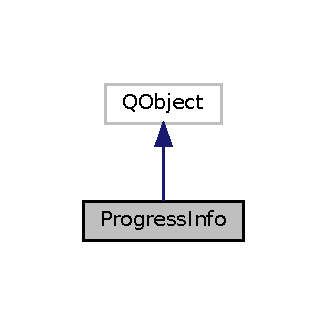
\includegraphics[width=157pt]{class_progress_info__inherit__graph}
\end{center}
\end{figure}


Collaboration diagram for Progress\+Info\+:
\nopagebreak
\begin{figure}[H]
\begin{center}
\leavevmode
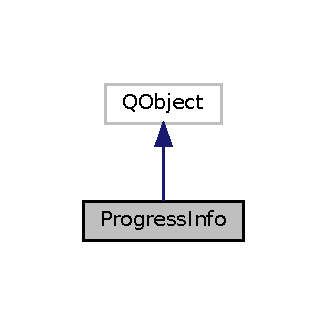
\includegraphics[width=157pt]{class_progress_info__coll__graph}
\end{center}
\end{figure}
\subsection*{Signals}
\begin{DoxyCompactItemize}
\item 
\mbox{\Hypertarget{class_progress_info_a73435651cd150eadc530c5727a5c21ca}\label{class_progress_info_a73435651cd150eadc530c5727a5c21ca}} 
void \mbox{\hyperlink{class_progress_info_a73435651cd150eadc530c5727a5c21ca}{progress\+Begin}} ()
\begin{DoxyCompactList}\small\item\em the progress begin \end{DoxyCompactList}\item 
\mbox{\Hypertarget{class_progress_info_a2d94864da963156de0d520ace292fcd6}\label{class_progress_info_a2d94864da963156de0d520ace292fcd6}} 
void \mbox{\hyperlink{class_progress_info_a2d94864da963156de0d520ace292fcd6}{progress\+End}} ()
\begin{DoxyCompactList}\small\item\em the progress is finished \end{DoxyCompactList}\item 
\mbox{\Hypertarget{class_progress_info_ab8abdf90f9a0061ebbeccf12eea339bf}\label{class_progress_info_ab8abdf90f9a0061ebbeccf12eea339bf}} 
void \mbox{\hyperlink{class_progress_info_ab8abdf90f9a0061ebbeccf12eea339bf}{progress\+Update}} ()
\begin{DoxyCompactList}\small\item\em the progress update \end{DoxyCompactList}\end{DoxyCompactItemize}
\subsection*{Public Member Functions}
\begin{DoxyCompactItemize}
\item 
void \mbox{\hyperlink{class_progress_info_ac67672902957c1cd4629d33ed1d76e81}{set\+Mark}} (unsigned int \mbox{\hyperlink{class_progress_info_a9d81184d13006d316c5c46133b7ff409}{mark}})
\begin{DoxyCompactList}\small\item\em set the maximum of the progress , emit progress\+Begin \end{DoxyCompactList}\item 
void \mbox{\hyperlink{class_progress_info_acbc2662a15cb1212bdbb223544f8b3d4}{set\+Progress}} (unsigned int \mbox{\hyperlink{class_progress_info_a0cf245dd88d85029da4952e1f74acc0f}{progress}})
\begin{DoxyCompactList}\small\item\em set the actual progress (between 0 and \+\_\+mark). emit progress\+Update \end{DoxyCompactList}\item 
\mbox{\Hypertarget{class_progress_info_af1f35fef86b813a7c9e60030806d9ffd}\label{class_progress_info_af1f35fef86b813a7c9e60030806d9ffd}} 
void \mbox{\hyperlink{class_progress_info_af1f35fef86b813a7c9e60030806d9ffd}{end\+Progress}} ()
\begin{DoxyCompactList}\small\item\em emit progress\+End \end{DoxyCompactList}\item 
unsigned int \mbox{\hyperlink{class_progress_info_a9d81184d13006d316c5c46133b7ff409}{mark}} () const
\begin{DoxyCompactList}\small\item\em get \+\_\+mark \end{DoxyCompactList}\item 
unsigned int \mbox{\hyperlink{class_progress_info_a0cf245dd88d85029da4952e1f74acc0f}{progress}} () const
\begin{DoxyCompactList}\small\item\em get \+\_\+progress \end{DoxyCompactList}\end{DoxyCompactItemize}


\subsection{Detailed Description}
Store the information of a progress and emit 3 signal (begin, update and end). 

\subsection{Member Function Documentation}
\mbox{\Hypertarget{class_progress_info_a9d81184d13006d316c5c46133b7ff409}\label{class_progress_info_a9d81184d13006d316c5c46133b7ff409}} 
\index{Progress\+Info@{Progress\+Info}!mark@{mark}}
\index{mark@{mark}!Progress\+Info@{Progress\+Info}}
\subsubsection{\texorpdfstring{mark()}{mark()}}
{\footnotesize\ttfamily unsigned int Progress\+Info\+::mark (\begin{DoxyParamCaption}{ }\end{DoxyParamCaption}) const}



get \+\_\+mark 

\begin{DoxyReturn}{Returns}
the maximum of the progress 
\end{DoxyReturn}
\mbox{\Hypertarget{class_progress_info_a0cf245dd88d85029da4952e1f74acc0f}\label{class_progress_info_a0cf245dd88d85029da4952e1f74acc0f}} 
\index{Progress\+Info@{Progress\+Info}!progress@{progress}}
\index{progress@{progress}!Progress\+Info@{Progress\+Info}}
\subsubsection{\texorpdfstring{progress()}{progress()}}
{\footnotesize\ttfamily unsigned int Progress\+Info\+::progress (\begin{DoxyParamCaption}{ }\end{DoxyParamCaption}) const}



get \+\_\+progress 

\begin{DoxyReturn}{Returns}
the actual progress 
\end{DoxyReturn}
\mbox{\Hypertarget{class_progress_info_ac67672902957c1cd4629d33ed1d76e81}\label{class_progress_info_ac67672902957c1cd4629d33ed1d76e81}} 
\index{Progress\+Info@{Progress\+Info}!set\+Mark@{set\+Mark}}
\index{set\+Mark@{set\+Mark}!Progress\+Info@{Progress\+Info}}
\subsubsection{\texorpdfstring{set\+Mark()}{setMark()}}
{\footnotesize\ttfamily void Progress\+Info\+::set\+Mark (\begin{DoxyParamCaption}\item[{unsigned int}]{mark }\end{DoxyParamCaption})}



set the maximum of the progress , emit progress\+Begin 


\begin{DoxyParams}{Parameters}
{\em mark} & the maximum of the progress \\
\hline
\end{DoxyParams}
\mbox{\Hypertarget{class_progress_info_acbc2662a15cb1212bdbb223544f8b3d4}\label{class_progress_info_acbc2662a15cb1212bdbb223544f8b3d4}} 
\index{Progress\+Info@{Progress\+Info}!set\+Progress@{set\+Progress}}
\index{set\+Progress@{set\+Progress}!Progress\+Info@{Progress\+Info}}
\subsubsection{\texorpdfstring{set\+Progress()}{setProgress()}}
{\footnotesize\ttfamily void Progress\+Info\+::set\+Progress (\begin{DoxyParamCaption}\item[{unsigned int}]{progress }\end{DoxyParamCaption})}



set the actual progress (between 0 and \+\_\+mark). emit progress\+Update 


\begin{DoxyParams}{Parameters}
{\em progress} & \\
\hline
\end{DoxyParams}


The documentation for this class was generated from the following files\+:\begin{DoxyCompactItemize}
\item 
src/progressinfo.\+h\item 
src/progressinfo.\+cpp\end{DoxyCompactItemize}

\hypertarget{class_shader}{}\section{Shader Class Reference}
\label{class_shader}\index{Shader@{Shader}}


The \mbox{\hyperlink{class_shader}{Shader}} class, opens, compiles and executes a vertex shader and a fragment shader.  




{\ttfamily \#include $<$shader.\+h$>$}

\subsection*{Public Member Functions}
\begin{DoxyCompactItemize}
\item 
\mbox{\hyperlink{class_shader_a03421a8419cdad4b84cf58ecdb156879}{Shader}} (const G\+Lchar $\ast$vertex\+Path, const G\+Lchar $\ast$fragment\+Path)
\begin{DoxyCompactList}\small\item\em Reads, compiles and stores the ID program of the shaders. \end{DoxyCompactList}\item 
\mbox{\Hypertarget{class_shader_a1712a23e6282d4cec7d95216bde65f6a}\label{class_shader_a1712a23e6282d4cec7d95216bde65f6a}} 
void \mbox{\hyperlink{class_shader_a1712a23e6282d4cec7d95216bde65f6a}{initialize}} ()
\begin{DoxyCompactList}\small\item\em Reads, compiles the vertex and the fragment shader. \end{DoxyCompactList}\item 
\mbox{\Hypertarget{class_shader_a870fa9f13d69e558815d6fd351a469dc}\label{class_shader_a870fa9f13d69e558815d6fd351a469dc}} 
void \mbox{\hyperlink{class_shader_a870fa9f13d69e558815d6fd351a469dc}{use}} ()
\begin{DoxyCompactList}\small\item\em activate the shader \end{DoxyCompactList}\item 
\mbox{\Hypertarget{class_shader_ad8368fcacdb176733217c6a15f3ad543}\label{class_shader_ad8368fcacdb176733217c6a15f3ad543}} 
void \mbox{\hyperlink{class_shader_ad8368fcacdb176733217c6a15f3ad543}{disable}} ()
\begin{DoxyCompactList}\small\item\em disable the shader \end{DoxyCompactList}\item 
unsigned int \mbox{\hyperlink{class_shader_a23a569879e4ede84a052c0d3a12ae3c0}{ID}} () const
\begin{DoxyCompactList}\small\item\em get the id program \end{DoxyCompactList}\item 
void \mbox{\hyperlink{class_shader_ab1a56d6c299bd7eaa18c2e142ef7bd9f}{set\+Bool}} (const std\+::string \&name, bool value) const
\begin{DoxyCompactList}\small\item\em set a boolean like a uniform value into the sharders \end{DoxyCompactList}\item 
void \mbox{\hyperlink{class_shader_ad362e2b654cd95a3574cd505411e41fd}{set\+Int}} (const std\+::string \&name, int value) const
\begin{DoxyCompactList}\small\item\em set a integer like a uniform value into the sharders \end{DoxyCompactList}\item 
void \mbox{\hyperlink{class_shader_afe7367621f74c2d26431d8ac15252bf3}{set\+Float}} (const std\+::string \&name, float value) const
\begin{DoxyCompactList}\small\item\em set a float like a uniform value into the sharders \end{DoxyCompactList}\item 
void \mbox{\hyperlink{class_shader_afd4d41322a1cdd1d5155bf124d19debf}{set\+Vec2}} (const std\+::string \&name, const glm\+::vec2 \&value) const
\begin{DoxyCompactList}\small\item\em set a 2D vector like a uniform value into the sharders \end{DoxyCompactList}\item 
void \mbox{\hyperlink{class_shader_afb91bc9e954bf590857c96ab1331b0ec}{set\+Vec2}} (const std\+::string \&name, float x, float y) const
\begin{DoxyCompactList}\small\item\em set a 2D vector like a uniform value into the sharders \end{DoxyCompactList}\item 
void \mbox{\hyperlink{class_shader_aeb021061c5d451329d92257b07dbfec3}{set\+Vec3}} (const std\+::string \&name, const glm\+::vec3 \&value) const
\begin{DoxyCompactList}\small\item\em set a 2D vector like a uniform value into the sharders \end{DoxyCompactList}\item 
void \mbox{\hyperlink{class_shader_a90092c25b7dc23964c465b93887300f9}{set\+Vec3}} (const std\+::string \&name, float x, float y, float z) const
\begin{DoxyCompactList}\small\item\em set a 3D vector like a uniform value into the sharders \end{DoxyCompactList}\item 
void \mbox{\hyperlink{class_shader_a79cbe674f6bf1a576a48045dcb924de5}{set\+Vec4}} (const std\+::string \&name, const glm\+::vec4 \&value) const
\begin{DoxyCompactList}\small\item\em set a 4D vector like a uniform value into the sharders \end{DoxyCompactList}\item 
void \mbox{\hyperlink{class_shader_a913e10fe2501b00746ae6901b97a1730}{set\+Vec4}} (const std\+::string \&name, float x, float y, float z, float w)
\begin{DoxyCompactList}\small\item\em set a 4D vector like a uniform value into the sharders \end{DoxyCompactList}\item 
void \mbox{\hyperlink{class_shader_a91a6ee79b959cacd618c9e29a5bbd732}{set\+Mat2}} (const std\+::string \&name, const glm\+::mat2 \&mat) const
\begin{DoxyCompactList}\small\item\em set a 2D matrix like a uniform value into the sharders \end{DoxyCompactList}\item 
void \mbox{\hyperlink{class_shader_a3e24fcad187493dfebaa12939072e91d}{set\+Mat3}} (const std\+::string \&name, const glm\+::mat3 \&mat) const
\begin{DoxyCompactList}\small\item\em set a 3D matrix like a uniform value into the sharders \end{DoxyCompactList}\item 
void \mbox{\hyperlink{class_shader_a8e711c96f3e1722cbfb88fde9478977c}{set\+Mat4}} (const std\+::string \&name, const glm\+::mat4 \&mat) const
\begin{DoxyCompactList}\small\item\em set a 4D matrix like a uniform value into the sharders \end{DoxyCompactList}\end{DoxyCompactItemize}


\subsection{Detailed Description}
The \mbox{\hyperlink{class_shader}{Shader}} class, opens, compiles and executes a vertex shader and a fragment shader. 

\subsection{Constructor \& Destructor Documentation}
\mbox{\Hypertarget{class_shader_a03421a8419cdad4b84cf58ecdb156879}\label{class_shader_a03421a8419cdad4b84cf58ecdb156879}} 
\index{Shader@{Shader}!Shader@{Shader}}
\index{Shader@{Shader}!Shader@{Shader}}
\subsubsection{\texorpdfstring{Shader()}{Shader()}}
{\footnotesize\ttfamily Shader\+::\+Shader (\begin{DoxyParamCaption}\item[{const G\+Lchar $\ast$}]{vertex\+Path,  }\item[{const G\+Lchar $\ast$}]{fragment\+Path }\end{DoxyParamCaption})}



Reads, compiles and stores the ID program of the shaders. 


\begin{DoxyParams}{Parameters}
{\em vertex\+Path} & \+: a path of a vertex shader \\
\hline
{\em fragment\+Path} & \+: a path of a fragment shader \\
\hline
\end{DoxyParams}


\subsection{Member Function Documentation}
\mbox{\Hypertarget{class_shader_a23a569879e4ede84a052c0d3a12ae3c0}\label{class_shader_a23a569879e4ede84a052c0d3a12ae3c0}} 
\index{Shader@{Shader}!ID@{ID}}
\index{ID@{ID}!Shader@{Shader}}
\subsubsection{\texorpdfstring{I\+D()}{ID()}}
{\footnotesize\ttfamily unsigned int Shader\+::\+ID (\begin{DoxyParamCaption}{ }\end{DoxyParamCaption}) const}



get the id program 

\begin{DoxyReturn}{Returns}
the id program 
\end{DoxyReturn}
\mbox{\Hypertarget{class_shader_ab1a56d6c299bd7eaa18c2e142ef7bd9f}\label{class_shader_ab1a56d6c299bd7eaa18c2e142ef7bd9f}} 
\index{Shader@{Shader}!set\+Bool@{set\+Bool}}
\index{set\+Bool@{set\+Bool}!Shader@{Shader}}
\subsubsection{\texorpdfstring{set\+Bool()}{setBool()}}
{\footnotesize\ttfamily void Shader\+::set\+Bool (\begin{DoxyParamCaption}\item[{const std\+::string \&}]{name,  }\item[{bool}]{value }\end{DoxyParamCaption}) const}



set a boolean like a uniform value into the sharders 


\begin{DoxyParams}{Parameters}
{\em name} & \+: the name of the boolean \\
\hline
{\em value} & \+: the value of the boolean \\
\hline
\end{DoxyParams}
\mbox{\Hypertarget{class_shader_afe7367621f74c2d26431d8ac15252bf3}\label{class_shader_afe7367621f74c2d26431d8ac15252bf3}} 
\index{Shader@{Shader}!set\+Float@{set\+Float}}
\index{set\+Float@{set\+Float}!Shader@{Shader}}
\subsubsection{\texorpdfstring{set\+Float()}{setFloat()}}
{\footnotesize\ttfamily void Shader\+::set\+Float (\begin{DoxyParamCaption}\item[{const std\+::string \&}]{name,  }\item[{float}]{value }\end{DoxyParamCaption}) const}



set a float like a uniform value into the sharders 


\begin{DoxyParams}{Parameters}
{\em name} & \+: the name of the float \\
\hline
{\em value} & \+: the value of the float \\
\hline
\end{DoxyParams}
\mbox{\Hypertarget{class_shader_ad362e2b654cd95a3574cd505411e41fd}\label{class_shader_ad362e2b654cd95a3574cd505411e41fd}} 
\index{Shader@{Shader}!set\+Int@{set\+Int}}
\index{set\+Int@{set\+Int}!Shader@{Shader}}
\subsubsection{\texorpdfstring{set\+Int()}{setInt()}}
{\footnotesize\ttfamily void Shader\+::set\+Int (\begin{DoxyParamCaption}\item[{const std\+::string \&}]{name,  }\item[{int}]{value }\end{DoxyParamCaption}) const}



set a integer like a uniform value into the sharders 


\begin{DoxyParams}{Parameters}
{\em name} & \+: the name of the integer \\
\hline
{\em value} & \+: the value of the integer \\
\hline
\end{DoxyParams}
\mbox{\Hypertarget{class_shader_a91a6ee79b959cacd618c9e29a5bbd732}\label{class_shader_a91a6ee79b959cacd618c9e29a5bbd732}} 
\index{Shader@{Shader}!set\+Mat2@{set\+Mat2}}
\index{set\+Mat2@{set\+Mat2}!Shader@{Shader}}
\subsubsection{\texorpdfstring{set\+Mat2()}{setMat2()}}
{\footnotesize\ttfamily void Shader\+::set\+Mat2 (\begin{DoxyParamCaption}\item[{const std\+::string \&}]{name,  }\item[{const glm\+::mat2 \&}]{mat }\end{DoxyParamCaption}) const}



set a 2D matrix like a uniform value into the sharders 


\begin{DoxyParams}{Parameters}
{\em name} & \+: the name of the 2D matrix \\
\hline
{\em value} & \+: the value of the 2D matrix \\
\hline
\end{DoxyParams}
\mbox{\Hypertarget{class_shader_a3e24fcad187493dfebaa12939072e91d}\label{class_shader_a3e24fcad187493dfebaa12939072e91d}} 
\index{Shader@{Shader}!set\+Mat3@{set\+Mat3}}
\index{set\+Mat3@{set\+Mat3}!Shader@{Shader}}
\subsubsection{\texorpdfstring{set\+Mat3()}{setMat3()}}
{\footnotesize\ttfamily void Shader\+::set\+Mat3 (\begin{DoxyParamCaption}\item[{const std\+::string \&}]{name,  }\item[{const glm\+::mat3 \&}]{mat }\end{DoxyParamCaption}) const}



set a 3D matrix like a uniform value into the sharders 


\begin{DoxyParams}{Parameters}
{\em name} & \+: the name of the 3D matrix \\
\hline
{\em value} & \+: the value of the 3D matrix \\
\hline
\end{DoxyParams}
\mbox{\Hypertarget{class_shader_a8e711c96f3e1722cbfb88fde9478977c}\label{class_shader_a8e711c96f3e1722cbfb88fde9478977c}} 
\index{Shader@{Shader}!set\+Mat4@{set\+Mat4}}
\index{set\+Mat4@{set\+Mat4}!Shader@{Shader}}
\subsubsection{\texorpdfstring{set\+Mat4()}{setMat4()}}
{\footnotesize\ttfamily void Shader\+::set\+Mat4 (\begin{DoxyParamCaption}\item[{const std\+::string \&}]{name,  }\item[{const glm\+::mat4 \&}]{mat }\end{DoxyParamCaption}) const}



set a 4D matrix like a uniform value into the sharders 


\begin{DoxyParams}{Parameters}
{\em name} & \+: the name of the 4D matrix \\
\hline
{\em value} & \+: the value of the 4D matrix \\
\hline
\end{DoxyParams}
\mbox{\Hypertarget{class_shader_afd4d41322a1cdd1d5155bf124d19debf}\label{class_shader_afd4d41322a1cdd1d5155bf124d19debf}} 
\index{Shader@{Shader}!set\+Vec2@{set\+Vec2}}
\index{set\+Vec2@{set\+Vec2}!Shader@{Shader}}
\subsubsection{\texorpdfstring{set\+Vec2()}{setVec2()}\hspace{0.1cm}{\footnotesize\ttfamily [1/2]}}
{\footnotesize\ttfamily void Shader\+::set\+Vec2 (\begin{DoxyParamCaption}\item[{const std\+::string \&}]{name,  }\item[{const glm\+::vec2 \&}]{value }\end{DoxyParamCaption}) const}



set a 2D vector like a uniform value into the sharders 


\begin{DoxyParams}{Parameters}
{\em name} & \+: the name of the 2D vector \\
\hline
{\em value} & \+: the value of the 2D vector \\
\hline
\end{DoxyParams}
\mbox{\Hypertarget{class_shader_afb91bc9e954bf590857c96ab1331b0ec}\label{class_shader_afb91bc9e954bf590857c96ab1331b0ec}} 
\index{Shader@{Shader}!set\+Vec2@{set\+Vec2}}
\index{set\+Vec2@{set\+Vec2}!Shader@{Shader}}
\subsubsection{\texorpdfstring{set\+Vec2()}{setVec2()}\hspace{0.1cm}{\footnotesize\ttfamily [2/2]}}
{\footnotesize\ttfamily void Shader\+::set\+Vec2 (\begin{DoxyParamCaption}\item[{const std\+::string \&}]{name,  }\item[{float}]{x,  }\item[{float}]{y }\end{DoxyParamCaption}) const}



set a 2D vector like a uniform value into the sharders 


\begin{DoxyParams}{Parameters}
{\em name} & \+: the name of the 2D vector \\
\hline
{\em x} & \+: the x value of the 2D vector \\
\hline
{\em y} & \+: the y value of the 2D vector \\
\hline
\end{DoxyParams}
\mbox{\Hypertarget{class_shader_aeb021061c5d451329d92257b07dbfec3}\label{class_shader_aeb021061c5d451329d92257b07dbfec3}} 
\index{Shader@{Shader}!set\+Vec3@{set\+Vec3}}
\index{set\+Vec3@{set\+Vec3}!Shader@{Shader}}
\subsubsection{\texorpdfstring{set\+Vec3()}{setVec3()}\hspace{0.1cm}{\footnotesize\ttfamily [1/2]}}
{\footnotesize\ttfamily void Shader\+::set\+Vec3 (\begin{DoxyParamCaption}\item[{const std\+::string \&}]{name,  }\item[{const glm\+::vec3 \&}]{value }\end{DoxyParamCaption}) const}



set a 2D vector like a uniform value into the sharders 


\begin{DoxyParams}{Parameters}
{\em name} & \+: the name of the 2D vector \\
\hline
{\em value} & \+: the value of the 2D vector \\
\hline
\end{DoxyParams}
\mbox{\Hypertarget{class_shader_a90092c25b7dc23964c465b93887300f9}\label{class_shader_a90092c25b7dc23964c465b93887300f9}} 
\index{Shader@{Shader}!set\+Vec3@{set\+Vec3}}
\index{set\+Vec3@{set\+Vec3}!Shader@{Shader}}
\subsubsection{\texorpdfstring{set\+Vec3()}{setVec3()}\hspace{0.1cm}{\footnotesize\ttfamily [2/2]}}
{\footnotesize\ttfamily void Shader\+::set\+Vec3 (\begin{DoxyParamCaption}\item[{const std\+::string \&}]{name,  }\item[{float}]{x,  }\item[{float}]{y,  }\item[{float}]{z }\end{DoxyParamCaption}) const}



set a 3D vector like a uniform value into the sharders 


\begin{DoxyParams}{Parameters}
{\em name} & \+: the name of the 3D vector \\
\hline
{\em x} & \+: the x value of the 3D vector \\
\hline
{\em y} & \+: the y value of the 3D vector \\
\hline
{\em z} & \+: the z value of the 3D vector \\
\hline
\end{DoxyParams}
\mbox{\Hypertarget{class_shader_a79cbe674f6bf1a576a48045dcb924de5}\label{class_shader_a79cbe674f6bf1a576a48045dcb924de5}} 
\index{Shader@{Shader}!set\+Vec4@{set\+Vec4}}
\index{set\+Vec4@{set\+Vec4}!Shader@{Shader}}
\subsubsection{\texorpdfstring{set\+Vec4()}{setVec4()}\hspace{0.1cm}{\footnotesize\ttfamily [1/2]}}
{\footnotesize\ttfamily void Shader\+::set\+Vec4 (\begin{DoxyParamCaption}\item[{const std\+::string \&}]{name,  }\item[{const glm\+::vec4 \&}]{value }\end{DoxyParamCaption}) const}



set a 4D vector like a uniform value into the sharders 


\begin{DoxyParams}{Parameters}
{\em name} & \+: the name of the 4D vector \\
\hline
{\em value} & \+: the value of the 4D vector \\
\hline
\end{DoxyParams}
\mbox{\Hypertarget{class_shader_a913e10fe2501b00746ae6901b97a1730}\label{class_shader_a913e10fe2501b00746ae6901b97a1730}} 
\index{Shader@{Shader}!set\+Vec4@{set\+Vec4}}
\index{set\+Vec4@{set\+Vec4}!Shader@{Shader}}
\subsubsection{\texorpdfstring{set\+Vec4()}{setVec4()}\hspace{0.1cm}{\footnotesize\ttfamily [2/2]}}
{\footnotesize\ttfamily void Shader\+::set\+Vec4 (\begin{DoxyParamCaption}\item[{const std\+::string \&}]{name,  }\item[{float}]{x,  }\item[{float}]{y,  }\item[{float}]{z,  }\item[{float}]{w }\end{DoxyParamCaption})}



set a 4D vector like a uniform value into the sharders 


\begin{DoxyParams}{Parameters}
{\em name} & \+: the name of the 4D vector \\
\hline
{\em x} & \+: the x value of the 4D vector \\
\hline
{\em y} & \+: the y value of the 4D vector \\
\hline
{\em z} & \+: the z value of the 4D vector \\
\hline
{\em w} & \+: the w value of the 4D vector \\
\hline
\end{DoxyParams}


The documentation for this class was generated from the following files\+:\begin{DoxyCompactItemize}
\item 
src/shader.\+h\item 
src/shader.\+cpp\end{DoxyCompactItemize}

\hypertarget{struct_texture}{}\section{Texture Struct Reference}
\label{struct_texture}\index{Texture@{Texture}}


A struct to store the id and the type of a texture.  




{\ttfamily \#include $<$model.\+h$>$}

\subsection*{Public Attributes}
\begin{DoxyCompactItemize}
\item 
unsigned int \mbox{\hyperlink{struct_texture_aed42161a5c00b6020c85833401da6da6}{id}}
\item 
std\+::string \mbox{\hyperlink{struct_texture_a916a835d009806f2a57546c7705942b1}{type}}
\end{DoxyCompactItemize}


\subsection{Detailed Description}
A struct to store the id and the type of a texture. 

\subsection{Member Data Documentation}
\mbox{\Hypertarget{struct_texture_aed42161a5c00b6020c85833401da6da6}\label{struct_texture_aed42161a5c00b6020c85833401da6da6}} 
\index{Texture@{Texture}!id@{id}}
\index{id@{id}!Texture@{Texture}}
\subsubsection{\texorpdfstring{id}{id}}
{\footnotesize\ttfamily unsigned int Texture\+::id}

ID of the texture assign by gl\+Gen\+Textures() \mbox{\Hypertarget{struct_texture_a916a835d009806f2a57546c7705942b1}\label{struct_texture_a916a835d009806f2a57546c7705942b1}} 
\index{Texture@{Texture}!type@{type}}
\index{type@{type}!Texture@{Texture}}
\subsubsection{\texorpdfstring{type}{type}}
{\footnotesize\ttfamily std\+::string Texture\+::type}

The type of the texture 

The documentation for this struct was generated from the following file\+:\begin{DoxyCompactItemize}
\item 
src/model.\+h\end{DoxyCompactItemize}

\hypertarget{class_track_ball}{}\section{Track\+Ball Class Reference}
\label{class_track_ball}\index{Track\+Ball@{Track\+Ball}}


A sphere that can move around his center.  




{\ttfamily \#include $<$trackball.\+h$>$}

\subsection*{Public Member Functions}
\begin{DoxyCompactItemize}
\item 
\mbox{\hyperlink{class_track_ball_a9e524069acc51788c7712765521bc3ce}{Track\+Ball}} (float radius, const glm\+::vec2 \&center)
\item 
\mbox{\hyperlink{class_track_ball_ae391da576b739343d488dbe80302cc0c}{Track\+Ball}} (const \mbox{\hyperlink{class_track_ball}{Track\+Ball}} \&t)
\item 
\mbox{\hyperlink{class_track_ball}{Track\+Ball}} \& \mbox{\hyperlink{class_track_ball_a8a34d15e31c43046f5e12e596ff91b63}{operator=}} (const \mbox{\hyperlink{class_track_ball}{Track\+Ball}} \&t)
\item 
void \mbox{\hyperlink{class_track_ball_a98dca62dce061a1f880278e55bbc1afb}{begin\+Tracking}} (const glm\+::vec2 \&pt)
\item 
glm\+::quat \mbox{\hyperlink{class_track_ball_aa562dadd39fcb9b859026ba14a5ea75f}{track}} (const glm\+::vec2 \&pt)
\item 
void \mbox{\hyperlink{class_track_ball_adf981d2f821a0ba5399289291d0dc646}{set\+Center}} (const glm\+::vec2 \&center)
\item 
void \mbox{\hyperlink{class_track_ball_ab4d35e045512cb2d6d1081f171fbf7d4}{set\+Radius}} (float radius)
\end{DoxyCompactItemize}


\subsection{Detailed Description}
A sphere that can move around his center. 

\subsection{Constructor \& Destructor Documentation}
\mbox{\Hypertarget{class_track_ball_a9e524069acc51788c7712765521bc3ce}\label{class_track_ball_a9e524069acc51788c7712765521bc3ce}} 
\index{Track\+Ball@{Track\+Ball}!Track\+Ball@{Track\+Ball}}
\index{Track\+Ball@{Track\+Ball}!Track\+Ball@{Track\+Ball}}
\subsubsection{\texorpdfstring{Track\+Ball()}{TrackBall()}\hspace{0.1cm}{\footnotesize\ttfamily [1/2]}}
{\footnotesize\ttfamily Track\+Ball\+::\+Track\+Ball (\begin{DoxyParamCaption}\item[{float}]{radius,  }\item[{const glm\+::vec2 \&}]{center }\end{DoxyParamCaption})}


\begin{DoxyParams}{Parameters}
{\em radius} & \\
\hline
{\em center} & \\
\hline
\end{DoxyParams}
\mbox{\Hypertarget{class_track_ball_ae391da576b739343d488dbe80302cc0c}\label{class_track_ball_ae391da576b739343d488dbe80302cc0c}} 
\index{Track\+Ball@{Track\+Ball}!Track\+Ball@{Track\+Ball}}
\index{Track\+Ball@{Track\+Ball}!Track\+Ball@{Track\+Ball}}
\subsubsection{\texorpdfstring{Track\+Ball()}{TrackBall()}\hspace{0.1cm}{\footnotesize\ttfamily [2/2]}}
{\footnotesize\ttfamily Track\+Ball\+::\+Track\+Ball (\begin{DoxyParamCaption}\item[{const \mbox{\hyperlink{class_track_ball}{Track\+Ball}} \&}]{t }\end{DoxyParamCaption})}


\begin{DoxyParams}{Parameters}
{\em t} & \\
\hline
\end{DoxyParams}


\subsection{Member Function Documentation}
\mbox{\Hypertarget{class_track_ball_a98dca62dce061a1f880278e55bbc1afb}\label{class_track_ball_a98dca62dce061a1f880278e55bbc1afb}} 
\index{Track\+Ball@{Track\+Ball}!begin\+Tracking@{begin\+Tracking}}
\index{begin\+Tracking@{begin\+Tracking}!Track\+Ball@{Track\+Ball}}
\subsubsection{\texorpdfstring{begin\+Tracking()}{beginTracking()}}
{\footnotesize\ttfamily void Track\+Ball\+::begin\+Tracking (\begin{DoxyParamCaption}\item[{const glm\+::vec2 \&}]{pt }\end{DoxyParamCaption})\hspace{0.3cm}{\ttfamily [inline]}}


\begin{DoxyParams}{Parameters}
{\em pt} & \\
\hline
\end{DoxyParams}
\mbox{\Hypertarget{class_track_ball_a8a34d15e31c43046f5e12e596ff91b63}\label{class_track_ball_a8a34d15e31c43046f5e12e596ff91b63}} 
\index{Track\+Ball@{Track\+Ball}!operator=@{operator=}}
\index{operator=@{operator=}!Track\+Ball@{Track\+Ball}}
\subsubsection{\texorpdfstring{operator=()}{operator=()}}
{\footnotesize\ttfamily \mbox{\hyperlink{class_track_ball}{Track\+Ball}} \& Track\+Ball\+::operator= (\begin{DoxyParamCaption}\item[{const \mbox{\hyperlink{class_track_ball}{Track\+Ball}} \&}]{t }\end{DoxyParamCaption})\hspace{0.3cm}{\ttfamily [inline]}}


\begin{DoxyParams}{Parameters}
{\em t} & \\
\hline
\end{DoxyParams}
\begin{DoxyReturn}{Returns}
\mbox{\hyperlink{class_track_ball}{Track\+Ball}} \&operator
\end{DoxyReturn}

\begin{DoxyParams}{Parameters}
{\em t} & \\
\hline
\end{DoxyParams}
\begin{DoxyReturn}{Returns}
\mbox{\hyperlink{class_track_ball}{Track\+Ball}} \&Track\+Ball\+::operator 
\end{DoxyReturn}
\mbox{\Hypertarget{class_track_ball_adf981d2f821a0ba5399289291d0dc646}\label{class_track_ball_adf981d2f821a0ba5399289291d0dc646}} 
\index{Track\+Ball@{Track\+Ball}!set\+Center@{set\+Center}}
\index{set\+Center@{set\+Center}!Track\+Ball@{Track\+Ball}}
\subsubsection{\texorpdfstring{set\+Center()}{setCenter()}}
{\footnotesize\ttfamily void Track\+Ball\+::set\+Center (\begin{DoxyParamCaption}\item[{const glm\+::vec2 \&}]{center }\end{DoxyParamCaption})\hspace{0.3cm}{\ttfamily [inline]}}


\begin{DoxyParams}{Parameters}
{\em center} & \\
\hline
\end{DoxyParams}
\mbox{\Hypertarget{class_track_ball_ab4d35e045512cb2d6d1081f171fbf7d4}\label{class_track_ball_ab4d35e045512cb2d6d1081f171fbf7d4}} 
\index{Track\+Ball@{Track\+Ball}!set\+Radius@{set\+Radius}}
\index{set\+Radius@{set\+Radius}!Track\+Ball@{Track\+Ball}}
\subsubsection{\texorpdfstring{set\+Radius()}{setRadius()}}
{\footnotesize\ttfamily void Track\+Ball\+::set\+Radius (\begin{DoxyParamCaption}\item[{float}]{radius }\end{DoxyParamCaption})\hspace{0.3cm}{\ttfamily [inline]}}


\begin{DoxyParams}{Parameters}
{\em radius} & \\
\hline
\end{DoxyParams}
\mbox{\Hypertarget{class_track_ball_aa562dadd39fcb9b859026ba14a5ea75f}\label{class_track_ball_aa562dadd39fcb9b859026ba14a5ea75f}} 
\index{Track\+Ball@{Track\+Ball}!track@{track}}
\index{track@{track}!Track\+Ball@{Track\+Ball}}
\subsubsection{\texorpdfstring{track()}{track()}}
{\footnotesize\ttfamily glm\+::quat Track\+Ball\+::track (\begin{DoxyParamCaption}\item[{const glm\+::vec2 \&}]{pt }\end{DoxyParamCaption})\hspace{0.3cm}{\ttfamily [inline]}}


\begin{DoxyParams}{Parameters}
{\em pt} & \\
\hline
\end{DoxyParams}
\begin{DoxyReturn}{Returns}
glm\+::quat 
\end{DoxyReturn}


The documentation for this class was generated from the following files\+:\begin{DoxyCompactItemize}
\item 
src/trackball.\+h\item 
src/trackball.\+cpp\end{DoxyCompactItemize}

\hypertarget{class_vertex}{}\section{Vertex Class Reference}
\label{class_vertex}\index{Vertex@{Vertex}}


A Type class that define a vertex with his position , his normal and his texture coordinates.  




{\ttfamily \#include $<$vertex.\+h$>$}

\subsection*{Public Member Functions}
\begin{DoxyCompactItemize}
\item 
\mbox{\hyperlink{class_vertex_a4688b182b5b52ed10c978f5c11399d1f}{Vertex}} (glm\+::vec3 position, glm\+::vec3 normal, glm\+::vec2 tex\+Coords)
\begin{DoxyCompactList}\small\item\em Constructor with 3 3D vectors. \end{DoxyCompactList}\item 
\mbox{\hyperlink{class_vertex_ac20c5ee4fd9eab3c9dbf36e0a3a5b276}{Vertex}} (float px, float py, float pz, float nx, float ny, float nz, float tu, float tv)
\begin{DoxyCompactList}\small\item\em Constructor with each value of each vector. \end{DoxyCompactList}\item 
\mbox{\hyperlink{class_vertex_a81b6330b9b8bf45e357b1c9d3c7d37dc}{Vertex}} (float px, float py, float pz, float tu, float tv)
\begin{DoxyCompactList}\small\item\em Constructor with position and texture coordinates , the normal is initialized to (0,0,0). \end{DoxyCompactList}\item 
\mbox{\hyperlink{class_vertex_a5833a02aa7d93a5fafb6d84f8065322f}{Vertex}} (float px, float py, float pz)
\begin{DoxyCompactList}\small\item\em Constructor with only the position, the normal is initialized to (0,0,0) and texture coordinates are initilized to 0. \end{DoxyCompactList}\item 
bool \mbox{\hyperlink{class_vertex_af8eb8e095d89b9ab47d1e8814d9e353b}{operator$<$}} (const \mbox{\hyperlink{class_vertex}{Vertex}} that) const
\begin{DoxyCompactList}\small\item\em test if that is superior to this \end{DoxyCompactList}\item 
\mbox{\Hypertarget{class_vertex_abc2531c8f9b2eed32478f4fba4603e88}\label{class_vertex_abc2531c8f9b2eed32478f4fba4603e88}} 
void \mbox{\hyperlink{class_vertex_abc2531c8f9b2eed32478f4fba4603e88}{print}} ()
\begin{DoxyCompactList}\small\item\em Print the actual vertex. \end{DoxyCompactList}\end{DoxyCompactItemize}
\subsection*{Public Attributes}
\begin{DoxyCompactItemize}
\item 
\mbox{\Hypertarget{class_vertex_abb3cfacd96b5955b0cec9359840ee49f}\label{class_vertex_abb3cfacd96b5955b0cec9359840ee49f}} 
glm\+::vec3 \mbox{\hyperlink{class_vertex_abb3cfacd96b5955b0cec9359840ee49f}{Position}}
\begin{DoxyCompactList}\small\item\em The position of the vertex. \end{DoxyCompactList}\item 
\mbox{\Hypertarget{class_vertex_a9ab4dc431b41509f0b1bb1a4bf09d4e2}\label{class_vertex_a9ab4dc431b41509f0b1bb1a4bf09d4e2}} 
glm\+::vec3 \mbox{\hyperlink{class_vertex_a9ab4dc431b41509f0b1bb1a4bf09d4e2}{Normal}}
\begin{DoxyCompactList}\small\item\em The normal of the vertex. \end{DoxyCompactList}\item 
\mbox{\Hypertarget{class_vertex_a921a513c1e6d1e63e99d477fa837a317}\label{class_vertex_a921a513c1e6d1e63e99d477fa837a317}} 
glm\+::vec2 \mbox{\hyperlink{class_vertex_a921a513c1e6d1e63e99d477fa837a317}{Tex\+Coords}}
\begin{DoxyCompactList}\small\item\em the texture coordinates of the vertex \end{DoxyCompactList}\end{DoxyCompactItemize}


\subsection{Detailed Description}
A Type class that define a vertex with his position , his normal and his texture coordinates. 

\subsection{Constructor \& Destructor Documentation}
\mbox{\Hypertarget{class_vertex_a4688b182b5b52ed10c978f5c11399d1f}\label{class_vertex_a4688b182b5b52ed10c978f5c11399d1f}} 
\index{Vertex@{Vertex}!Vertex@{Vertex}}
\index{Vertex@{Vertex}!Vertex@{Vertex}}
\subsubsection{\texorpdfstring{Vertex()}{Vertex()}\hspace{0.1cm}{\footnotesize\ttfamily [1/4]}}
{\footnotesize\ttfamily Vertex\+::\+Vertex (\begin{DoxyParamCaption}\item[{glm\+::vec3}]{position,  }\item[{glm\+::vec3}]{normal,  }\item[{glm\+::vec2}]{tex\+Coords }\end{DoxyParamCaption})}



Constructor with 3 3D vectors. 


\begin{DoxyParams}{Parameters}
{\em position} & 3D vectors that define the position. \\
\hline
{\em normal} & 3D vectors that define the normal. \\
\hline
{\em tex\+Coords} & 2D vectors that define the texture coordinates. \\
\hline
\end{DoxyParams}
\mbox{\Hypertarget{class_vertex_ac20c5ee4fd9eab3c9dbf36e0a3a5b276}\label{class_vertex_ac20c5ee4fd9eab3c9dbf36e0a3a5b276}} 
\index{Vertex@{Vertex}!Vertex@{Vertex}}
\index{Vertex@{Vertex}!Vertex@{Vertex}}
\subsubsection{\texorpdfstring{Vertex()}{Vertex()}\hspace{0.1cm}{\footnotesize\ttfamily [2/4]}}
{\footnotesize\ttfamily Vertex\+::\+Vertex (\begin{DoxyParamCaption}\item[{float}]{px,  }\item[{float}]{py,  }\item[{float}]{pz,  }\item[{float}]{nx,  }\item[{float}]{ny,  }\item[{float}]{nz,  }\item[{float}]{tu,  }\item[{float}]{tv }\end{DoxyParamCaption})}



Constructor with each value of each vector. 


\begin{DoxyParams}{Parameters}
{\em px} & \+: the x of the position. \\
\hline
{\em py} & \+: the y of the position. \\
\hline
{\em pz} & \+: the z of the position. \\
\hline
{\em nx} & \+: the x of the normal. \\
\hline
{\em ny} & \+: the y of the normal. \\
\hline
{\em nz} & \+: the z of the normal. \\
\hline
{\em tu} & \+: the u of the texture coordinates. \\
\hline
{\em tv} & \+: the v of the texture coordinates. \\
\hline
\end{DoxyParams}
\mbox{\Hypertarget{class_vertex_a81b6330b9b8bf45e357b1c9d3c7d37dc}\label{class_vertex_a81b6330b9b8bf45e357b1c9d3c7d37dc}} 
\index{Vertex@{Vertex}!Vertex@{Vertex}}
\index{Vertex@{Vertex}!Vertex@{Vertex}}
\subsubsection{\texorpdfstring{Vertex()}{Vertex()}\hspace{0.1cm}{\footnotesize\ttfamily [3/4]}}
{\footnotesize\ttfamily Vertex\+::\+Vertex (\begin{DoxyParamCaption}\item[{float}]{px,  }\item[{float}]{py,  }\item[{float}]{pz,  }\item[{float}]{tu,  }\item[{float}]{tv }\end{DoxyParamCaption})}



Constructor with position and texture coordinates , the normal is initialized to (0,0,0). 


\begin{DoxyParams}{Parameters}
{\em px} & \+: the x of the position. \\
\hline
{\em py} & \+: the y of the position. \\
\hline
{\em pz} & \+: the z of the position. \\
\hline
{\em tu} & \+: the u of the texture coordinates. \\
\hline
{\em tv} & \+: the v of the texture coordinates. \\
\hline
\end{DoxyParams}
\mbox{\Hypertarget{class_vertex_a5833a02aa7d93a5fafb6d84f8065322f}\label{class_vertex_a5833a02aa7d93a5fafb6d84f8065322f}} 
\index{Vertex@{Vertex}!Vertex@{Vertex}}
\index{Vertex@{Vertex}!Vertex@{Vertex}}
\subsubsection{\texorpdfstring{Vertex()}{Vertex()}\hspace{0.1cm}{\footnotesize\ttfamily [4/4]}}
{\footnotesize\ttfamily Vertex\+::\+Vertex (\begin{DoxyParamCaption}\item[{float}]{px,  }\item[{float}]{py,  }\item[{float}]{pz }\end{DoxyParamCaption})}



Constructor with only the position, the normal is initialized to (0,0,0) and texture coordinates are initilized to 0. 


\begin{DoxyParams}{Parameters}
{\em px} & \+: the x of the position. \\
\hline
{\em py} & \+: the y of the position. \\
\hline
{\em pz} & \+: the z of the position. \\
\hline
\end{DoxyParams}


\subsection{Member Function Documentation}
\mbox{\Hypertarget{class_vertex_af8eb8e095d89b9ab47d1e8814d9e353b}\label{class_vertex_af8eb8e095d89b9ab47d1e8814d9e353b}} 
\index{Vertex@{Vertex}!operator$<$@{operator$<$}}
\index{operator$<$@{operator$<$}!Vertex@{Vertex}}
\subsubsection{\texorpdfstring{operator$<$()}{operator<()}}
{\footnotesize\ttfamily bool Vertex\+::operator$<$ (\begin{DoxyParamCaption}\item[{const \mbox{\hyperlink{class_vertex}{Vertex}}}]{that }\end{DoxyParamCaption}) const}



test if that is superior to this 


\begin{DoxyParams}{Parameters}
{\em that} & \+: a vertex \\
\hline
\end{DoxyParams}
\begin{DoxyReturn}{Returns}
true if that $>$ this, else otherwise. 
\end{DoxyReturn}


The documentation for this class was generated from the following files\+:\begin{DoxyCompactItemize}
\item 
src/vertex.\+h\item 
src/vertex.\+cpp\end{DoxyCompactItemize}

\hypertarget{class_viewer}{}\section{Viewer Class Reference}
\label{class_viewer}\index{Viewer@{Viewer}}


The Open GL widget , init open\+GL, setup a model, a camera, a light and shaders and draw it.  




{\ttfamily \#include $<$viewer.\+h$>$}



Inheritance diagram for Viewer\+:
\nopagebreak
\begin{figure}[H]
\begin{center}
\leavevmode
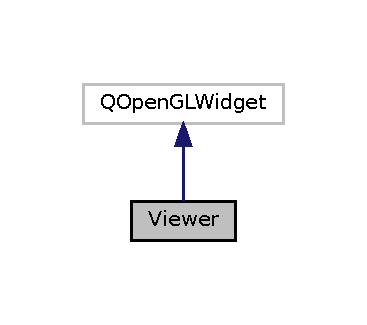
\includegraphics[width=176pt]{class_viewer__inherit__graph}
\end{center}
\end{figure}


Collaboration diagram for Viewer\+:
\nopagebreak
\begin{figure}[H]
\begin{center}
\leavevmode
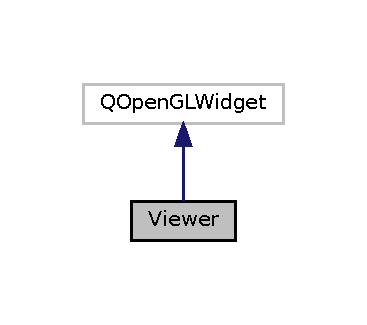
\includegraphics[width=176pt]{class_viewer__coll__graph}
\end{center}
\end{figure}
\subsection*{Public Member Functions}
\begin{DoxyCompactItemize}
\item 
\mbox{\hyperlink{class_viewer_a6a1f845092e1d4407adabb550e40431b}{Viewer}} (Q\+Widget $\ast$parent=0)
\begin{DoxyCompactList}\small\item\em Classic Q\+Widget constructor, set up a Q\+Surface\+Format. \end{DoxyCompactList}\item 
\mbox{\Hypertarget{class_viewer_a0acb833945df75a7547a8aa43d10511a}\label{class_viewer_a0acb833945df75a7547a8aa43d10511a}} 
virtual void \mbox{\hyperlink{class_viewer_a0acb833945df75a7547a8aa43d10511a}{paint\+GL}} ()
\begin{DoxyCompactList}\small\item\em Main loop of rendering. \end{DoxyCompactList}\item 
\mbox{\Hypertarget{class_viewer_a56ba84e76143655770007b413c56bb2d}\label{class_viewer_a56ba84e76143655770007b413c56bb2d}} 
virtual void \mbox{\hyperlink{class_viewer_a56ba84e76143655770007b413c56bb2d}{initialize\+GL}} ()
\begin{DoxyCompactList}\small\item\em initialize open\+Gl and the different element of viewer (model, camera, shader). \end{DoxyCompactList}\item 
virtual void \mbox{\hyperlink{class_viewer_a03c6a6d6c43c9fbcc26d11cb944d4875}{resize\+GL}} (int width, int height)
\begin{DoxyCompactList}\small\item\em Resize the widget. \end{DoxyCompactList}\item 
virtual void \mbox{\hyperlink{class_viewer_a1e9fa3e1484e31424260db80826d24a5}{key\+Press\+Event}} (Q\+Key\+Event $\ast$ke)
\begin{DoxyCompactList}\small\item\em Intercepts the imput of the Keybord and do something depeding on the pressed key \+: \end{DoxyCompactList}\item 
virtual void \mbox{\hyperlink{class_viewer_aa8cd58104b20ce3ba5ec502eb09afca6}{mouse\+Press\+Event}} (Q\+Mouse\+Event $\ast$me)
\begin{DoxyCompactList}\small\item\em Intercepts the imput of the mousse and do something depeding on the pressed key. \end{DoxyCompactList}\item 
virtual void \mbox{\hyperlink{class_viewer_a3d05b37233c2d97f4e68b2ee5a1277e2}{mouse\+Move\+Event}} (Q\+Mouse\+Event $\ast$me)
\begin{DoxyCompactList}\small\item\em Intercepts the movements of the mouss when a button is pressed and do something depeding the button pressed. \end{DoxyCompactList}\item 
bool \mbox{\hyperlink{class_viewer_a1a35d9603576f7c9a1895a6311ad81d8}{load\+Model\+From\+File}} (const Q\+String\+List \&file\+Names)
\begin{DoxyCompactList}\small\item\em check and copy a stack file in \+\_\+filepaths. \end{DoxyCompactList}\item 
\mbox{\hyperlink{class_progress_info}{Progress\+Info}} $\ast$ \mbox{\hyperlink{class_viewer_a7990e46887a50148c6dda326484c1996}{progress\+Info}} () const
\begin{DoxyCompactList}\small\item\em get \+\_\+progress\+Info. \end{DoxyCompactList}\end{DoxyCompactItemize}


\subsection{Detailed Description}
The Open GL widget , init open\+GL, setup a model, a camera, a light and shaders and draw it. 

\subsection{Constructor \& Destructor Documentation}
\mbox{\Hypertarget{class_viewer_a6a1f845092e1d4407adabb550e40431b}\label{class_viewer_a6a1f845092e1d4407adabb550e40431b}} 
\index{Viewer@{Viewer}!Viewer@{Viewer}}
\index{Viewer@{Viewer}!Viewer@{Viewer}}
\subsubsection{\texorpdfstring{Viewer()}{Viewer()}}
{\footnotesize\ttfamily Viewer\+::\+Viewer (\begin{DoxyParamCaption}\item[{Q\+Widget $\ast$}]{parent = {\ttfamily 0} }\end{DoxyParamCaption})}



Classic Q\+Widget constructor, set up a Q\+Surface\+Format. 


\begin{DoxyParams}{Parameters}
{\em parent} & the Q\+Widget parent of \mbox{\hyperlink{class_viewer}{Viewer}}. \\
\hline
\end{DoxyParams}


\subsection{Member Function Documentation}
\mbox{\Hypertarget{class_viewer_a1e9fa3e1484e31424260db80826d24a5}\label{class_viewer_a1e9fa3e1484e31424260db80826d24a5}} 
\index{Viewer@{Viewer}!key\+Press\+Event@{key\+Press\+Event}}
\index{key\+Press\+Event@{key\+Press\+Event}!Viewer@{Viewer}}
\subsubsection{\texorpdfstring{key\+Press\+Event()}{keyPressEvent()}}
{\footnotesize\ttfamily void Viewer\+::key\+Press\+Event (\begin{DoxyParamCaption}\item[{Q\+Key\+Event $\ast$}]{ke }\end{DoxyParamCaption})\hspace{0.3cm}{\ttfamily [virtual]}}



Intercepts the imput of the Keybord and do something depeding on the pressed key \+: 

-\/i \+: init the camera, -\/k \+: reload the shader 
\begin{DoxyParams}{Parameters}
{\em ke} & the key pressed \\
\hline
\end{DoxyParams}
\mbox{\Hypertarget{class_viewer_a1a35d9603576f7c9a1895a6311ad81d8}\label{class_viewer_a1a35d9603576f7c9a1895a6311ad81d8}} 
\index{Viewer@{Viewer}!load\+Model\+From\+File@{load\+Model\+From\+File}}
\index{load\+Model\+From\+File@{load\+Model\+From\+File}!Viewer@{Viewer}}
\subsubsection{\texorpdfstring{load\+Model\+From\+File()}{loadModelFromFile()}}
{\footnotesize\ttfamily bool Viewer\+::load\+Model\+From\+File (\begin{DoxyParamCaption}\item[{const Q\+String\+List \&}]{file\+Names }\end{DoxyParamCaption})}



check and copy a stack file in \+\_\+filepaths. 


\begin{DoxyParams}{Parameters}
{\em file\+Names} & a stack of path file. \\
\hline
\end{DoxyParams}
\begin{DoxyReturn}{Returns}
return true if the file\+Names are correct (.obj or .asc). 
\end{DoxyReturn}
\mbox{\Hypertarget{class_viewer_a3d05b37233c2d97f4e68b2ee5a1277e2}\label{class_viewer_a3d05b37233c2d97f4e68b2ee5a1277e2}} 
\index{Viewer@{Viewer}!mouse\+Move\+Event@{mouse\+Move\+Event}}
\index{mouse\+Move\+Event@{mouse\+Move\+Event}!Viewer@{Viewer}}
\subsubsection{\texorpdfstring{mouse\+Move\+Event()}{mouseMoveEvent()}}
{\footnotesize\ttfamily void Viewer\+::mouse\+Move\+Event (\begin{DoxyParamCaption}\item[{Q\+Mouse\+Event $\ast$}]{me }\end{DoxyParamCaption})\hspace{0.3cm}{\ttfamily [virtual]}}



Intercepts the movements of the mouss when a button is pressed and do something depeding the button pressed. 

-\/\+Left and Mid button \+: move the camera. -\/\+Right button \+: move the light. 
\begin{DoxyParams}{Parameters}
{\em me} & the button pressed. \\
\hline
\end{DoxyParams}
\mbox{\Hypertarget{class_viewer_aa8cd58104b20ce3ba5ec502eb09afca6}\label{class_viewer_aa8cd58104b20ce3ba5ec502eb09afca6}} 
\index{Viewer@{Viewer}!mouse\+Press\+Event@{mouse\+Press\+Event}}
\index{mouse\+Press\+Event@{mouse\+Press\+Event}!Viewer@{Viewer}}
\subsubsection{\texorpdfstring{mouse\+Press\+Event()}{mousePressEvent()}}
{\footnotesize\ttfamily void Viewer\+::mouse\+Press\+Event (\begin{DoxyParamCaption}\item[{Q\+Mouse\+Event $\ast$}]{me }\end{DoxyParamCaption})\hspace{0.3cm}{\ttfamily [virtual]}}



Intercepts the imput of the mousse and do something depeding on the pressed key. 


\begin{DoxyItemize}
\item Left button \+: move the camera.
\begin{DoxyItemize}
\item Mid button \+: zoom the camera.
\item Right button \+: move the light. 
\begin{DoxyParams}{Parameters}
{\em me} & the button pressed. \\
\hline
\end{DoxyParams}

\end{DoxyItemize}
\end{DoxyItemize}\mbox{\Hypertarget{class_viewer_a7990e46887a50148c6dda326484c1996}\label{class_viewer_a7990e46887a50148c6dda326484c1996}} 
\index{Viewer@{Viewer}!progress\+Info@{progress\+Info}}
\index{progress\+Info@{progress\+Info}!Viewer@{Viewer}}
\subsubsection{\texorpdfstring{progress\+Info()}{progressInfo()}}
{\footnotesize\ttfamily \mbox{\hyperlink{class_progress_info}{Progress\+Info}} $\ast$ Viewer\+::progress\+Info (\begin{DoxyParamCaption}{ }\end{DoxyParamCaption}) const}



get \+\_\+progress\+Info. 

\begin{DoxyReturn}{Returns}
the state of the progress of the mesh\+Loader. 
\end{DoxyReturn}
\mbox{\Hypertarget{class_viewer_a03c6a6d6c43c9fbcc26d11cb944d4875}\label{class_viewer_a03c6a6d6c43c9fbcc26d11cb944d4875}} 
\index{Viewer@{Viewer}!resize\+GL@{resize\+GL}}
\index{resize\+GL@{resize\+GL}!Viewer@{Viewer}}
\subsubsection{\texorpdfstring{resize\+G\+L()}{resizeGL()}}
{\footnotesize\ttfamily void Viewer\+::resize\+GL (\begin{DoxyParamCaption}\item[{int}]{width,  }\item[{int}]{height }\end{DoxyParamCaption})\hspace{0.3cm}{\ttfamily [virtual]}}



Resize the widget. 


\begin{DoxyParams}{Parameters}
{\em width} & \+: the new width of the widget. \\
\hline
{\em height} & \+: the new height of the widget. \\
\hline
\end{DoxyParams}


The documentation for this class was generated from the following files\+:\begin{DoxyCompactItemize}
\item 
src/viewer.\+h\item 
src/viewer.\+cpp\end{DoxyCompactItemize}

\chapter{File Documentation}
\hypertarget{camera_8h}{}\section{src/camera.h File Reference}
\label{camera_8h}\index{src/camera.\+h@{src/camera.\+h}}
{\ttfamily \#include \char`\"{}trackball.\+h\char`\"{}}\newline
{\ttfamily \#include $<$glm/glm.\+hpp$>$}\newline
{\ttfamily \#include $<$glm/gtc/matrix\+\_\+transform.\+hpp$>$}\newline
{\ttfamily \#include $<$glm/gtc/matrix\+\_\+inverse.\+hpp$>$}\newline
{\ttfamily \#include $<$glm/gtc/type\+\_\+ptr.\+hpp$>$}\newline
{\ttfamily \#include $<$glm/gtx/string\+\_\+cast.\+hpp$>$}\newline
{\ttfamily \#include $<$math.\+h$>$}\newline
Include dependency graph for camera.\+h\+:
\nopagebreak
\begin{figure}[H]
\begin{center}
\leavevmode
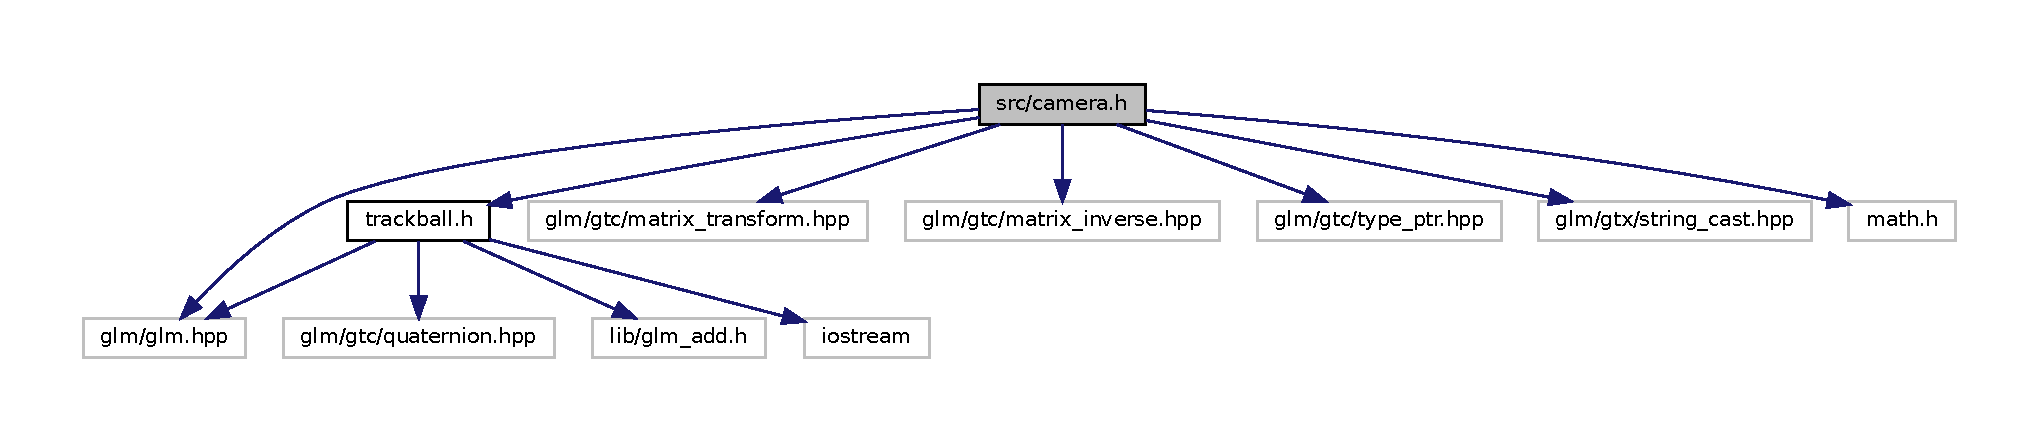
\includegraphics[width=350pt]{camera_8h__incl}
\end{center}
\end{figure}
This graph shows which files directly or indirectly include this file\+:
\nopagebreak
\begin{figure}[H]
\begin{center}
\leavevmode
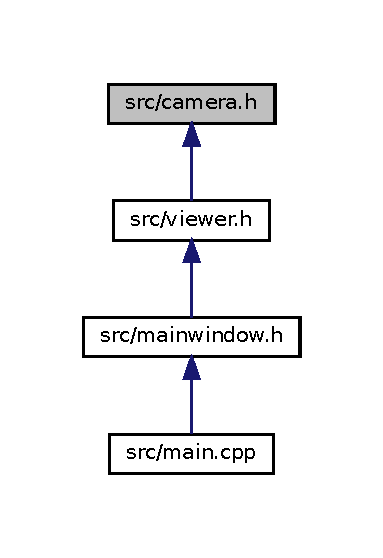
\includegraphics[width=184pt]{camera_8h__dep__incl}
\end{center}
\end{figure}
\subsection*{Classes}
\begin{DoxyCompactItemize}
\item 
class \mbox{\hyperlink{class_camera}{Camera}}
\begin{DoxyCompactList}\small\item\em Define a camera link to a trackball for move the model arround the trackball. Compute model-\/view matrix, projection matrix and normal matrix. ! The center must be (0,0,0) (B\+UG). \end{DoxyCompactList}\end{DoxyCompactItemize}


\subsection{Detailed Description}
\begin{DoxyAuthor}{Author}
Romain Vergne 
\end{DoxyAuthor}
\begin{DoxyVersion}{Version}
1.\+0 
\end{DoxyVersion}
\begin{DoxyDate}{Date}
26/02/2018 
\end{DoxyDate}

\hypertarget{main_8cpp}{}\section{src/main.cpp File Reference}
\label{main_8cpp}\index{src/main.\+cpp@{src/main.\+cpp}}


Application to generate a mountain panorama in the style of Pierre Novat.  


{\ttfamily \#include \char`\"{}mainwindow.\+h\char`\"{}}\newline
{\ttfamily \#include $<$qapplication.\+h$>$}\newline
Include dependency graph for main.\+cpp\+:
\nopagebreak
\begin{figure}[H]
\begin{center}
\leavevmode
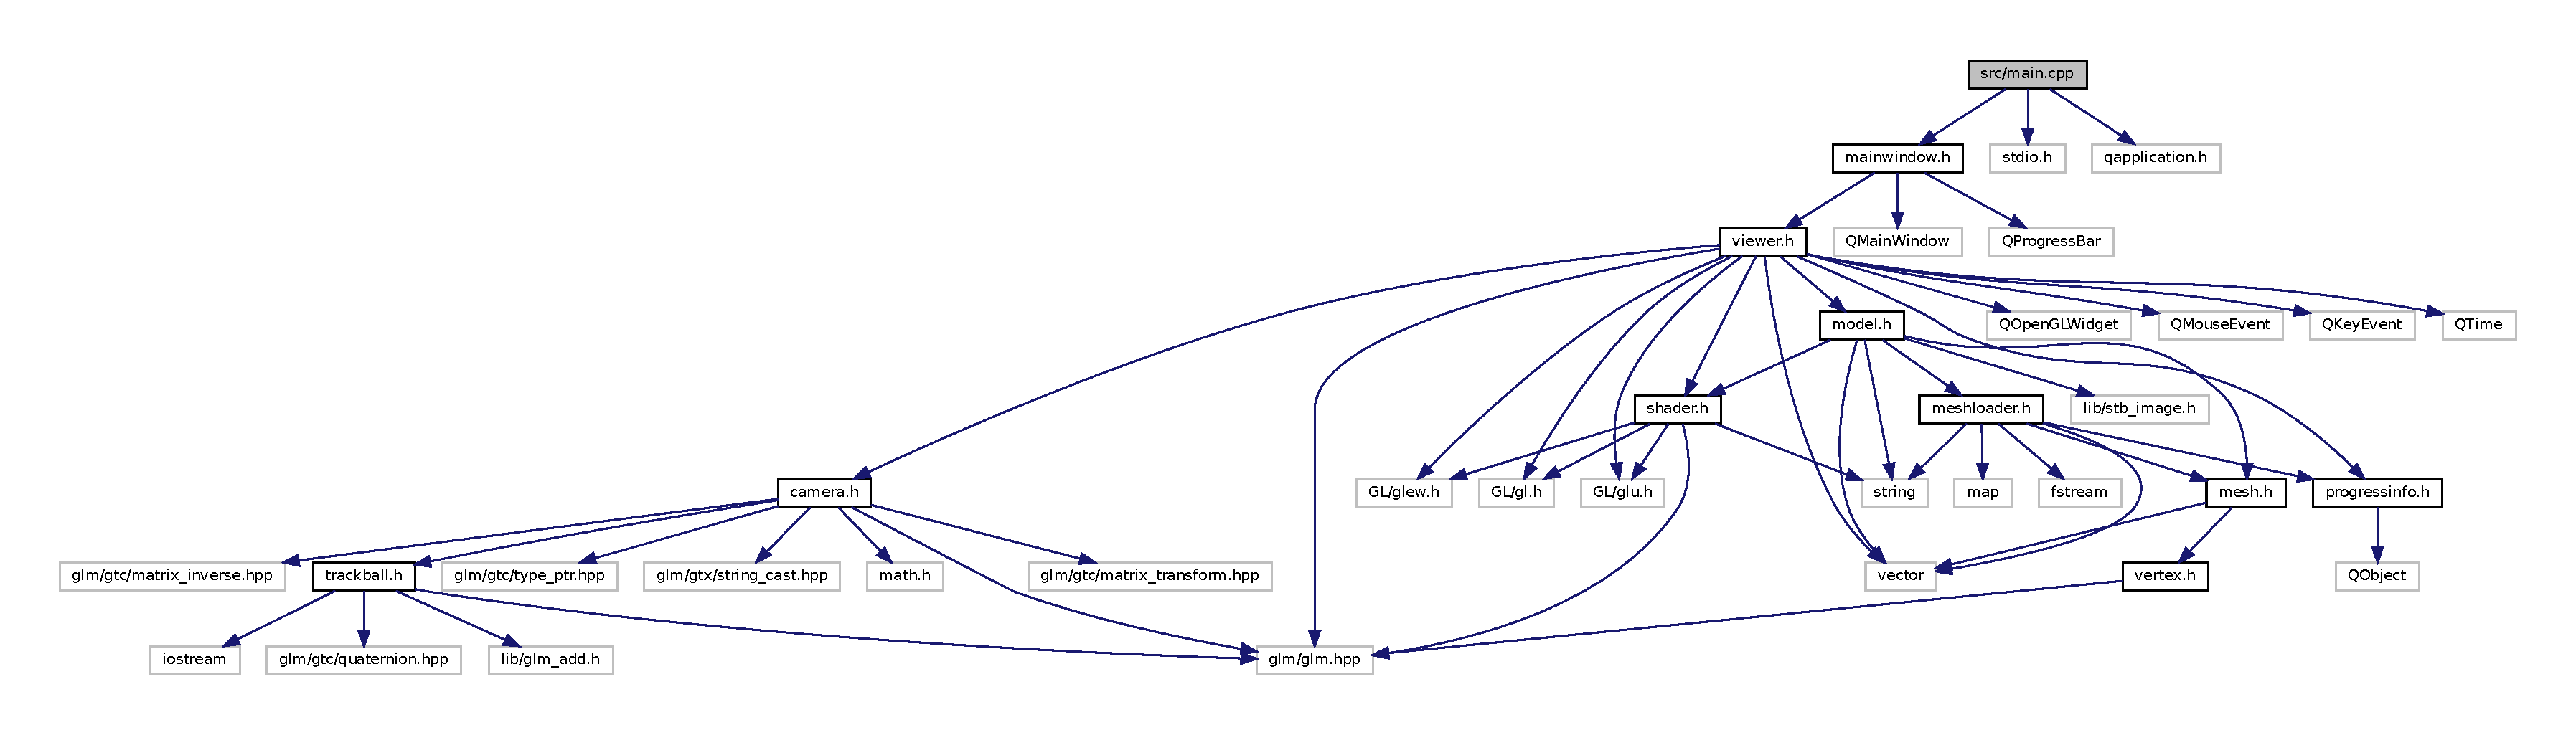
\includegraphics[width=350pt]{main_8cpp__incl}
\end{center}
\end{figure}
\subsection*{Functions}
\begin{DoxyCompactItemize}
\item 
int \mbox{\hyperlink{main_8cpp_a3c04138a5bfe5d72780bb7e82a18e627}{main}} (int argc, char $\ast$$\ast$argv)
\begin{DoxyCompactList}\small\item\em main create the app and the mainwindow \end{DoxyCompactList}\end{DoxyCompactItemize}


\subsection{Detailed Description}
Application to generate a mountain panorama in the style of Pierre Novat. 

\begin{DoxyAuthor}{Author}
Jonathan Granier 
\end{DoxyAuthor}
\begin{DoxyVersion}{Version}
1.\+0 
\end{DoxyVersion}
\begin{DoxyDate}{Date}
26/02/2018 
\end{DoxyDate}


\subsection{Function Documentation}
\mbox{\Hypertarget{main_8cpp_a3c04138a5bfe5d72780bb7e82a18e627}\label{main_8cpp_a3c04138a5bfe5d72780bb7e82a18e627}} 
\index{main.\+cpp@{main.\+cpp}!main@{main}}
\index{main@{main}!main.\+cpp@{main.\+cpp}}
\subsubsection{\texorpdfstring{main()}{main()}}
{\footnotesize\ttfamily int main (\begin{DoxyParamCaption}\item[{int}]{argc,  }\item[{char $\ast$$\ast$}]{argv }\end{DoxyParamCaption})}



main create the app and the mainwindow 


\begin{DoxyParams}{Parameters}
{\em argc} & Useless \\
\hline
{\em argv} & Useless \\
\hline
\end{DoxyParams}
\begin{DoxyReturn}{Returns}
Show Q\+Application.\+exec() return. 
\end{DoxyReturn}

%--- End generated contents ---

% Index
\backmatter
\newpage
\phantomsection
\clearemptydoublepage
\addcontentsline{toc}{chapter}{Index}
\printindex

\end{document}
